\documentclass[a4paper,12pt,english]{article}
\usepackage{glossaries}
\usepackage[T1]{fontenc}
\usepackage{babel}
\usepackage{graphicx}
\usepackage[table,xcdraw]{xcolor}
\usepackage{hyperref}
\usepackage{blindtext}
\usepackage{geometry}
\usepackage{parskip}
\usepackage{mathtools}
\usepackage{siunitx}
\usepackage{listings}
\usepackage{csquotes}
\usepackage{caption}
\usepackage{subcaption}
\usepackage{comment}
\usepackage{pdfpages}
\usepackage[useregional]{datetime2}
\usepackage{amsmath} % for the equation* environment
\usepackage{float}
\usepackage{pict2e}
\usepackage{fixltx2e}
\usepackage{tocloft}
\usepackage{graphicx}
\usepackage{xcolor}
\usepackage{float}
\usepackage{textgreek}
\usepackage{colortbl}
\usepackage{multirow}


%%gmedina solution
\newcommand{\listequationsname}{List of equations}
\newlistof{myequations}{equ}{\listequationsname}
\newcommand{\myequations}[1]{%
\addcontentsline{equ}{myequations}{\protect\numberline{\theequation}#1}\par}
\setlength{\cftmyequationsnumwidth}{2.5em}% Width of equation number in List of Equations

\DeclareRobustCommand{\slashcirc}{{\mathpalette\doslashcirc\relax}}

\makeatletter
\newcommand\doslashcirc[2]{%
  \sbox\z@{$#1\m@th\circ$}%
  \setlength\unitlength{\wd\z@}
  \begin{picture}(1,1)
  \roundcap
  \put(0,0){\box\z@}
  \put(0,0){\line(1,1){1}}
  \end{picture}%
}
\makeatother


\definecolor{stmblue}{RGB}{0,114,198}    % Adjusted STM32 blue color
\definecolor{stmgray}{RGB}{128,128,128}
\definecolor{stmgreen}{RGB}{34,177,76}    % Adjusted STM32 green color
\definecolor{stmorange}{RGB}{255,140,0}
\definecolor{codegreen}{rgb}{0,0.6,0}
\definecolor{codegray}{rgb}{0.5,0.5,0.5}
\definecolor{codepurple}{rgb}{0.58,0,0.82}

\lstset{
  language=C,
  basicstyle=\ttfamily\footnotesize,
  keywordstyle=\color{stmblue},
  stringstyle=\color{stmgreen},
  commentstyle=\color{stmgray},
  moredelim=[s][\color{stmorange}]{\#}{\ },
  frame=tb,
  tabsize=4,
  showstringspaces=false,
  breaklines=true,
  numbers=left,
  numberstyle=\tiny\color{stmgray},
  numbersep=5pt,
  extendedchars=true,
}

\lstdefinestyle{STM32}
{
    commentstyle=\color{codegreen},
    keywordstyle=\color{blue},
    numberstyle=\tiny\color{codegray},
    stringstyle=\color{codepurple},
    basicstyle=\ttfamily\small,
    breakatwhitespace=false,
    breaklines=true,
    captionpos=b,
    keepspaces=true,
    numbers=left,
    numbersep=5pt,
    showspaces=false,
    showstringspaces=false,
    showtabs=false,
    tabsize=2,
}



\usepackage[
    backend=biber,
    backref=true,
    backrefstyle=none,
    sortcites=true,
    sorting=none,
    doi=false, % doi informatie wordt niet weergegeven
    %uniquename=true,
    %uniquelist=true,
    maxcitenames=3,
    %issn=false, werkt niet
    language=american
]{biblatex}
\addbibresource{information/Sources.bib}
\DefineBibliographyStrings{english}{
    backrefpage = {page},
    backrefpages = {page},
}
\makeglossaries
\definecolor{Grey1}{HTML}{343434}
\graphicspath{{./img}}
 \geometry{
 a4paper,
 total={170mm,257mm},
 left=20mm,
 top=20mm,
 }
\hypersetup{
    colorlinks=true,
    linkcolor=blue,
    filecolor=magenta,      
    urlcolor=cyan,
    pdftitle={Overleaf Example},
    pdfpagemode=FullScreen,
    }


\begin{document}

\title{

\includegraphics[width=3.5in]{img/Logo/Logo.png} \\
\vspace*{1in}
\textbf{Project 4}\\
\textit{Testing report}\\
Version 1
}
\author{
\vspace*{0.5in} \\
  Written by:\\
  Laurens van der Drift\\
  Justin van der Reijden\\
  Luuk van Kappel\\
  Marnix Harmsen\\
		\vspace*{0.2in} \\
		The Hague University of Applied Sciences\\
        \textbf{Electrical Engineering}\\
        Delft, The Netherlands
       } 
\maketitle

\phantomsection
\section*{Version History} \addcontentsline{toc}{section}{Version History}

\begin{table}[h]
\begin{tabular}{|l|l|l|l|}
\hline
\rowcolor[HTML]{4472C4} 
{\color[HTML]{FFFFFF} \textbf{Version}} &
  {\color[HTML]{FFFFFF} \textbf{Date}} &
  {\color[HTML]{FFFFFF} \textbf{Changes}} &
  {\color[HTML]{FFFFFF} \textbf{Author}} \\ \hline
\rowcolor[HTML]{D9E1F2} 
1.0 &
  \multicolumn{1}{c|}{\cellcolor[HTML]{D9E1F2}25-04-2024} &
 N.v.t. &
  Alset Innovations \\ \hline

% \rowcolor[HTML]{FFFFFF} 
% 2.0 &
%   \multicolumn{1}{c|}{\cellcolor[HTML]{FFFFFF}7-4-2023} &
%  Feedback van FeedbackFruits toegepast &
%   Infra   Vroom \\ \hline

% \rowcolor[HTML]{D9E1F2} 
% 3.0 &
%   \multicolumn{1}{c|}{\cellcolor[HTML]{D9E1F2}4-6-2023} &
%  Bijgewerkt voor Assessment 3 &
%   Infra   Vroom \\ \hline

\end{tabular}
\end{table}

\phantomsection
\addcontentsline{toc}{section}{List of Figures}
\listoffigures

\newpage
\tableofcontents
% %\addcontentsline{toc}{section}{Verklarende Woordenlijst}
\printglossaries
\newglossaryentry{tender}
{
    name=\textit{tender},
    description={De inschrijving om op een kavel een wind turbine park te bouwen.}
}

% \phantomsection
\addcontentsline{toc}{section}{List of Figures}
\listoffigures

% \newpage
\tableofcontents

%% Use Arabic numerals for the page numbers of the chapters.
% \mainmatter %% fix dit MARNIX

% \section{STM32F411CEU6} \label{section:STM32F411CEU6}
\subsection{Why this MCU?} \label{subsection:Why_this_MCU}
The selection of the STM32F411CEU6 was driven by a desire to explore alternatives to the Pi Zero commonly used in similar projects. As pioneers in adopting this microcontroller, we are venturing into uncharted territory.
% Delving into the intricacies of our decision, let's explore the schematic in \autoref{fig:Blackpill_STM32F411CEU6_Schematic}.
\begin{figure}[H]
    \centering
    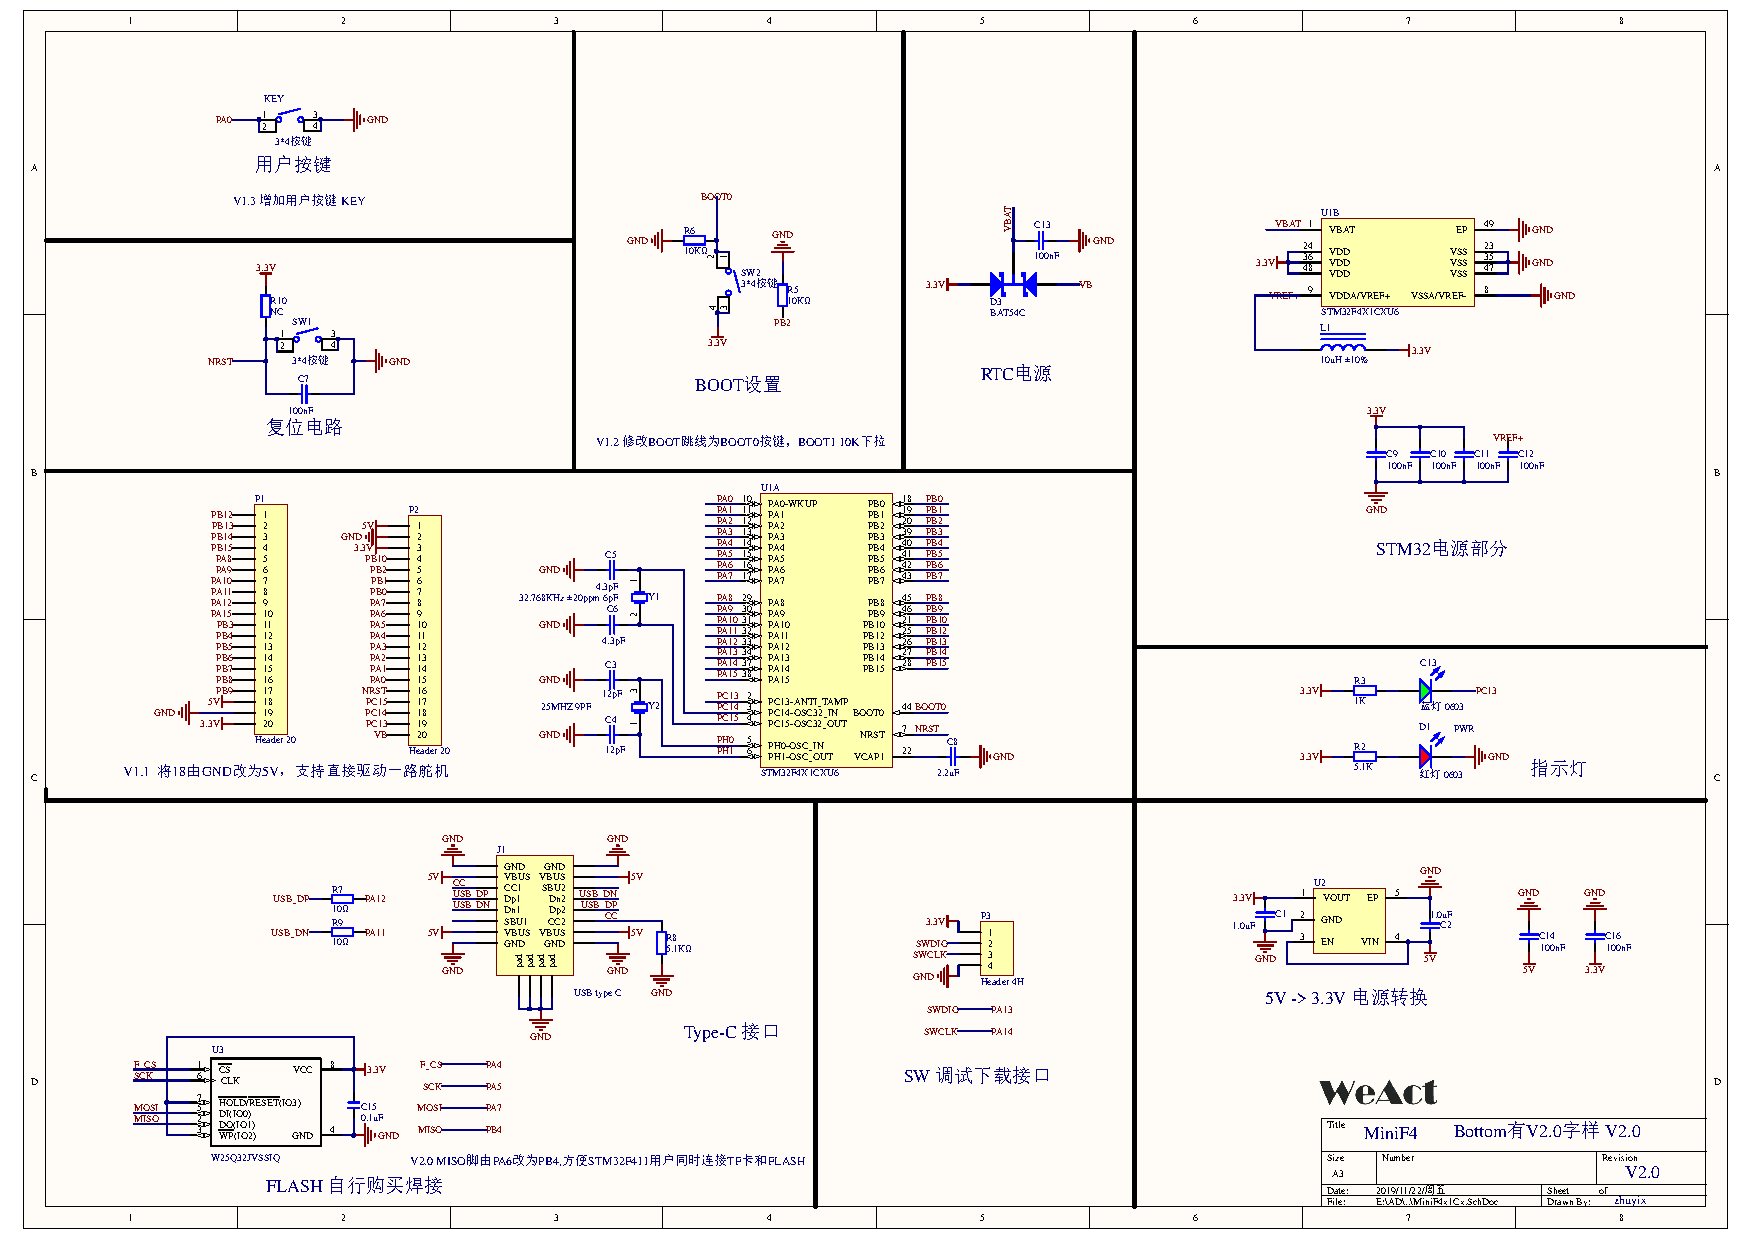
\includegraphics[width=1\linewidth]{img//blackpill/original-schematic-STM32F411CEU6_WeAct_Black_Pill_V2.0.pdf}
    \caption{Blackpill STM32F411CEU6 Schematic}
    \label{fig:Blackpill_STM32F411CEU6_Schematic}
\end{figure}
\begin{itemize}
    \item \textbf{Circuit with Buttons:} The schematic reveals a carefully designed circuit accommodating essential buttons - Key, Switch, and Boot - not crucial since we aren't using the onboard bootloader.

    \item \textbf{Real-Time Clock (RTC):} A dedicated circuit for real-time clock functionality ensures precise timing and synchronization within our motor control system.

    \item \textbf{STM32F411CEU6 Pinout:} The MCU itself is dissected with a pinout, providing insights into the connections and functionalities of each pin.

    \item \textbf{Voltage Regulator:} The presence of a voltage regulator ensures stable and reliable power distribution throughout the system.

    \item \textbf{Additional Circuits:} Beyond these components, the schematic highlights several other circuits vital for the holistic functionality of our design.
\end{itemize}

Moving from the abstract schematic to the tangible layout, the dimensions in \autoref{fig:Blackpill_STM32F411CEU6_Dimensions} depict the spatial arrangement of each component. Assembled into a cohesive unit, the complete PCB with the integrated STM32F411CEU6 is visualized in \autoref{fig:Blackpill_STM32F411CEU6_Picture}.
\begin{figure}[H]
    \centering
    \begin{subfigure}{0.48\textwidth}
        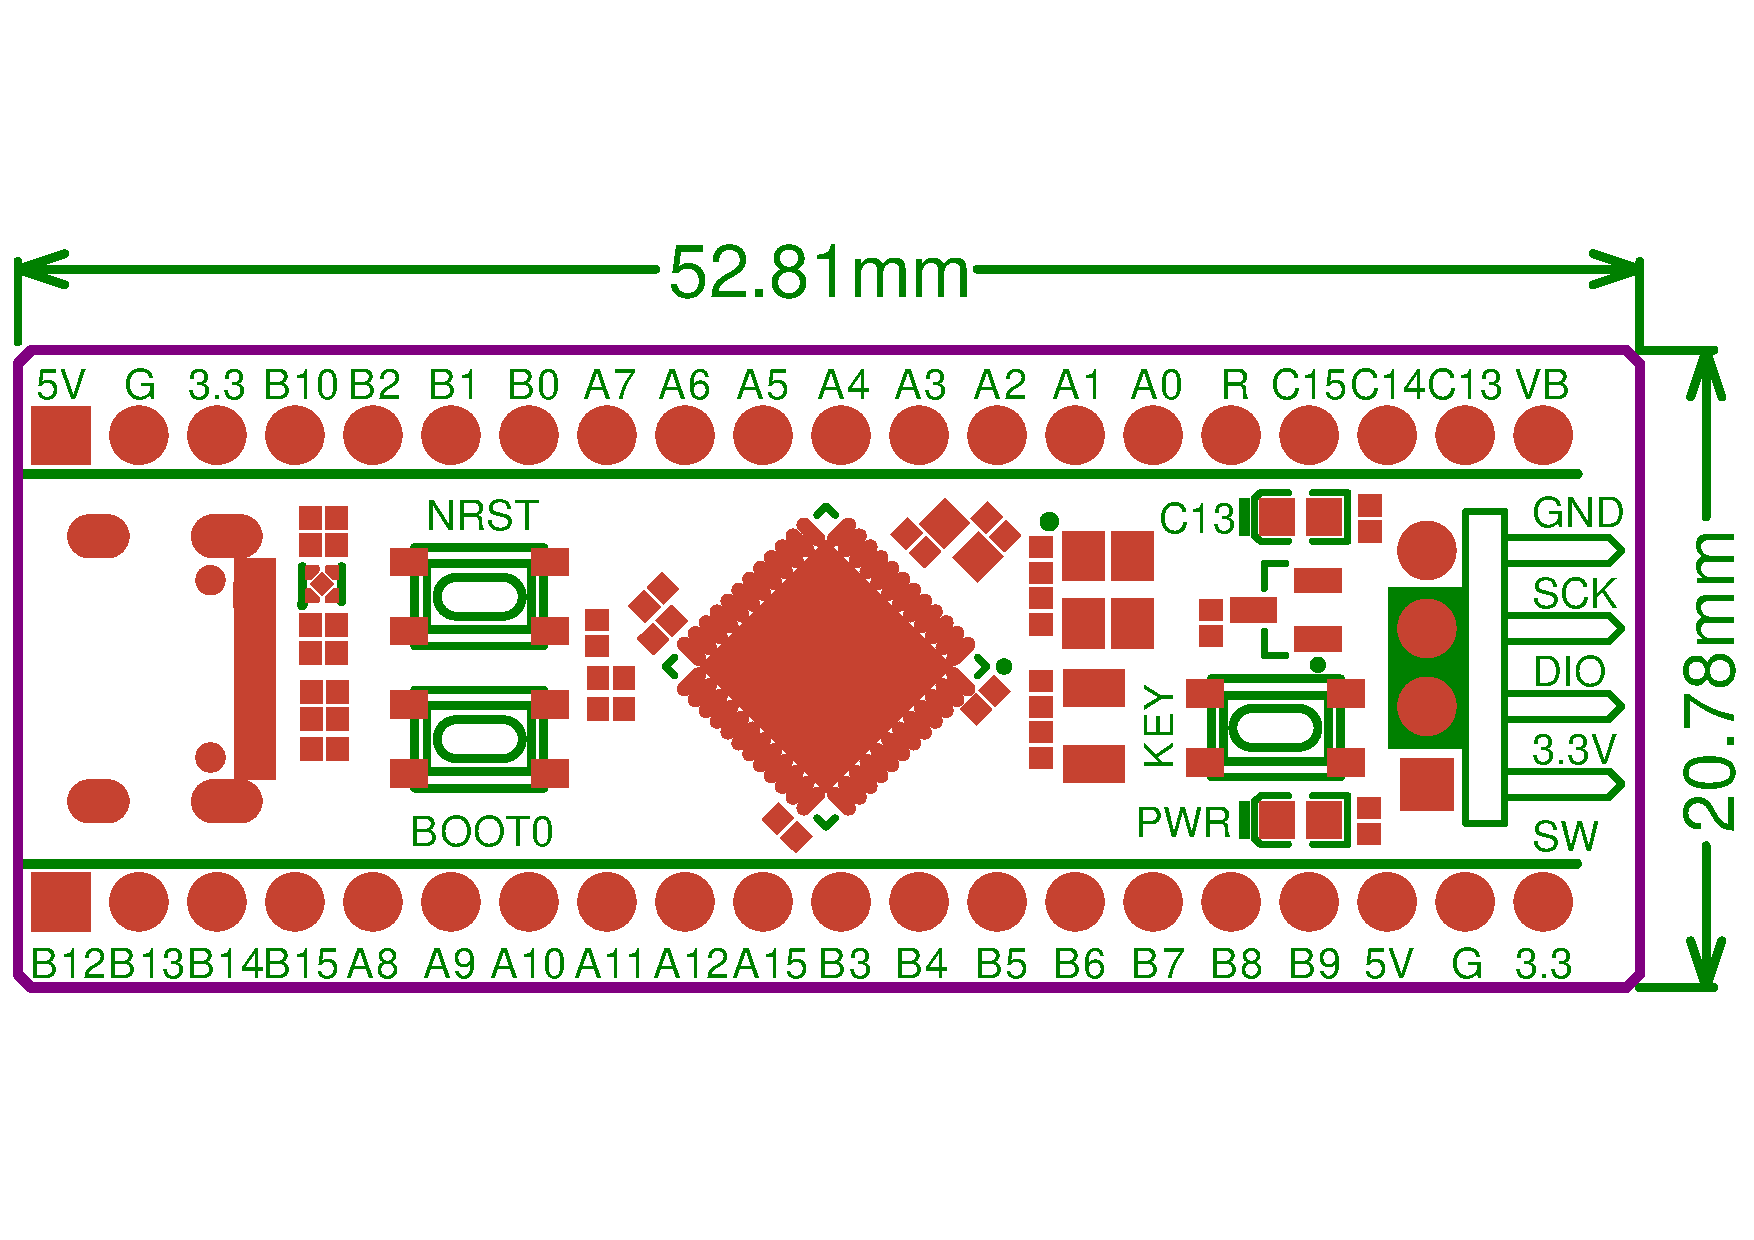
\includegraphics[width=\linewidth]{img/blackpill/original-dimensions-STM32F411CEU6_WeAct_Black_Pill_V2.0.pdf}
        \caption{Blackpill STM32F411CEU6 Dimensions}
        \label{fig:Blackpill_STM32F411CEU6_Dimensions}
    \end{subfigure}
    \hfill
    \begin{subfigure}{0.48\textwidth}
        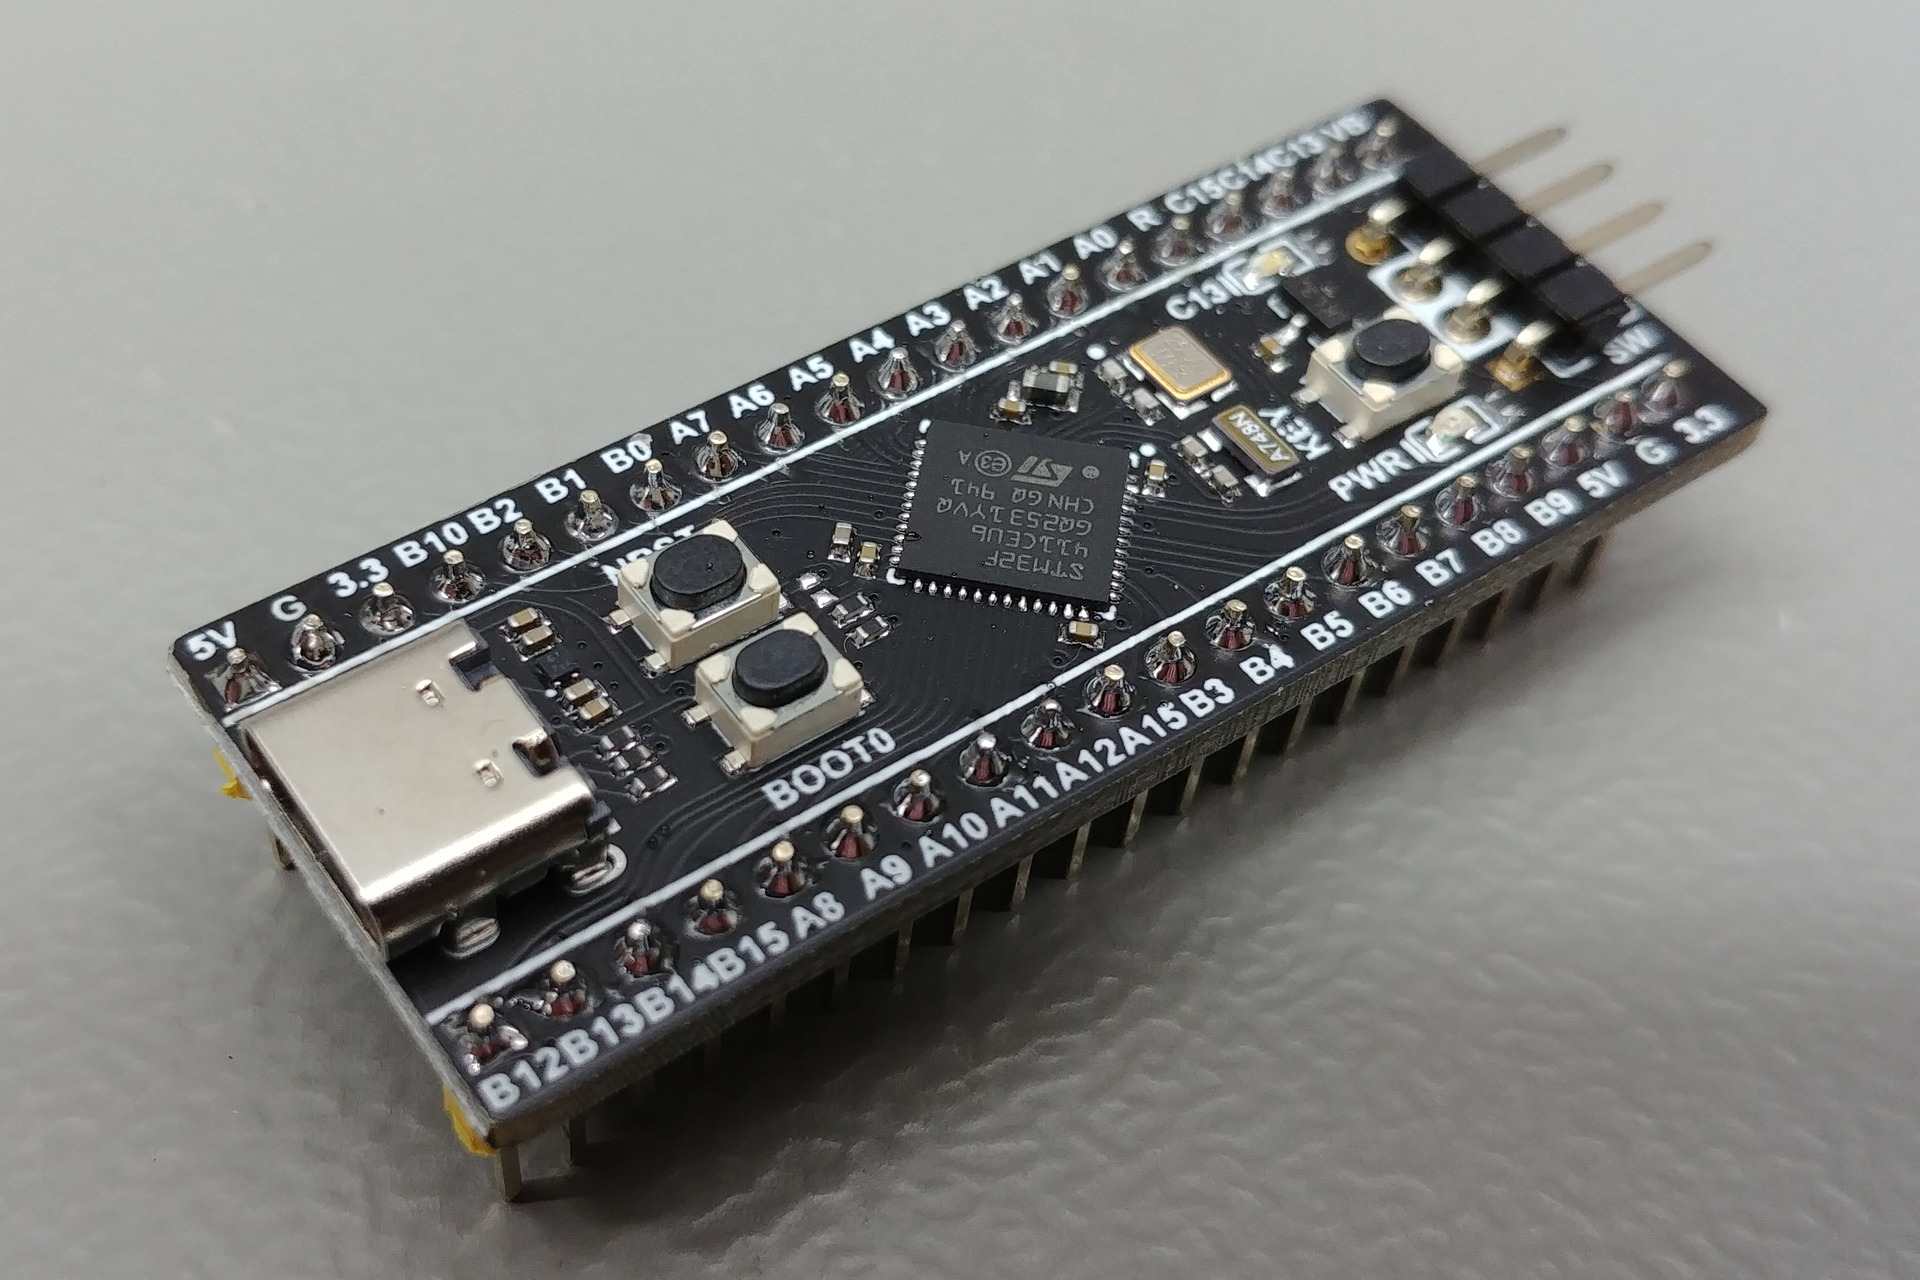
\includegraphics[width=\linewidth]{img/blackpill/STM32F411CEU6_WeAct_Black_Pill_V2.0-1.jpg}
    \caption{Blackpill STM32F411CEU6 Picture}
    \label{fig:Blackpill_STM32F411CEU6_Picture}
    \end{subfigure}
      \caption{Blackpill STM32F411CEU6}
  \label{fig:Blackpill STM32F411CEU6}
\end{figure}
In order to facilitate integration into our PCB design software, footprints and 3D models were developed for the component. Initially, KiCad was chosen for designing the model (see Figure \ref{fig:KiCadModel}) and footprint (see Figure \ref{fig:KiCadFootprint}), owing to our familiarity with the software. Subsequently, following consultation with Ad van den Bergh\cite{Adje}, we transitioned to using Altium Designer (refer to Figure \ref{fig:AltiumModel} \& \ref{fig:AltiumFootprint}). The creation of these models allows for seamless incorporation of the Blackpill breakout board into our custom PCB design.


\begin{figure}[H]
    \centering
    \begin{subfigure}{0.2\textwidth}
        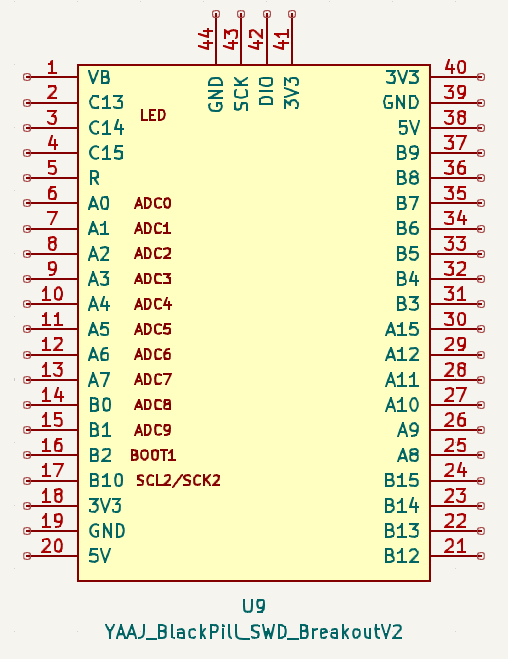
\includegraphics[width=\linewidth]{img//blackpill/KiCadMODEL.png}
        \caption{KiCad Model}
        \label{fig:KiCadModel}
    \end{subfigure}
    \hfill
    \begin{subfigure}{0.1\textwidth}
        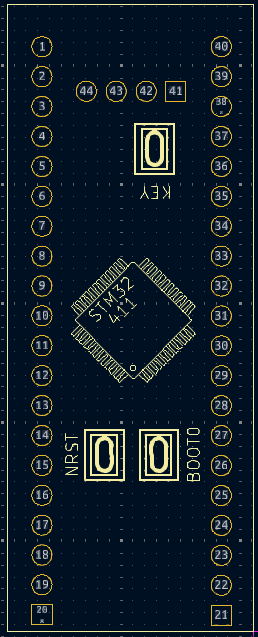
\includegraphics[width=\linewidth]{img//blackpill/KiCadFOOTPRINT1.png}
    \caption{KiCad Footprint}
    \label{fig:KiCadFootprint}
    \end{subfigure}
        \hfill
    \begin{subfigure}{0.2\textwidth}
        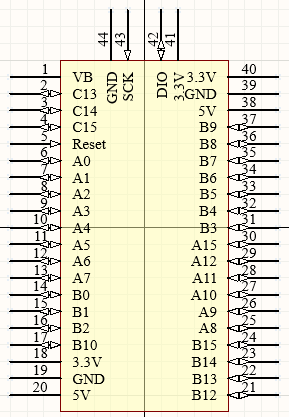
\includegraphics[width=\linewidth]{img//blackpill/AltiumMODEL.png}
        \caption{Altium Model}
        \label{fig:AltiumModel}
    \end{subfigure}
    \hfill
    \begin{subfigure}{0.2\textwidth}
        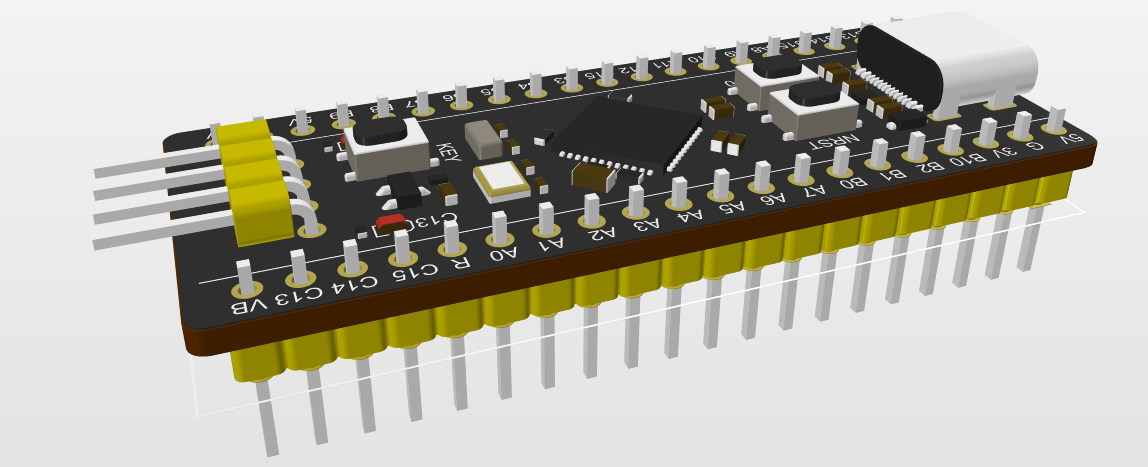
\includegraphics[width=\linewidth]{img//blackpill/AltiumFOOTPRINT.png}
    \caption{Altium Footprint}
    \label{fig:AltiumFootprint}
    \end{subfigure}
      \caption{Models\&Footprints}
  \label{fig:KiCadPCB}
\end{figure}



\section{Testing}
\subsection{Gate driver}\label{Gate driver}
In the initial phase of testing, the focus was on evaluating the gate drivers. Extensive testing and measurements were conducted. Initially, the IRS2004SPBF\cite{infineon-irs2004-datasheet} was utilized due to the sinusoidal signal being sent from the STM32F411\cite{stm32-base-board} to the gate drivers. However, both the code and hardware lacked optimization, leading to rapid heating of the BLDC motor\cite{reichelt-motor-datasheet} and increased current consumption(3+ amps) even under no load conditions, as illustrated in \autoref{fig:BLDCHEAT}. Subsequently, a shift in approach was made, opting for a block signal with the IRS2001SPBF\cite{infineon-irs2001-datasheet} gate driver. Although improved results were observed, the motor still exhibited some warmth, albeit less pronounced. To delve deeper into signal processing, the decision was made to alter the bootstrap resistors from 5 ohms to 1 ohm, effectively mitigating the occurrence of a small short (\autoref{fig:smallshort}). This adjustment proved to be pivotal. As a result, the BLDC motor\cite{reichelt-motor-datasheet} can now operate for 5 minutes at 4800 RPM without exceeding 50 degrees Celsius and staying below 250 mA, marking a significant achievement.
\begin{figure}[H]
    \centering
    \hfill
    \begin{subfigure}{0.42\textwidth}
        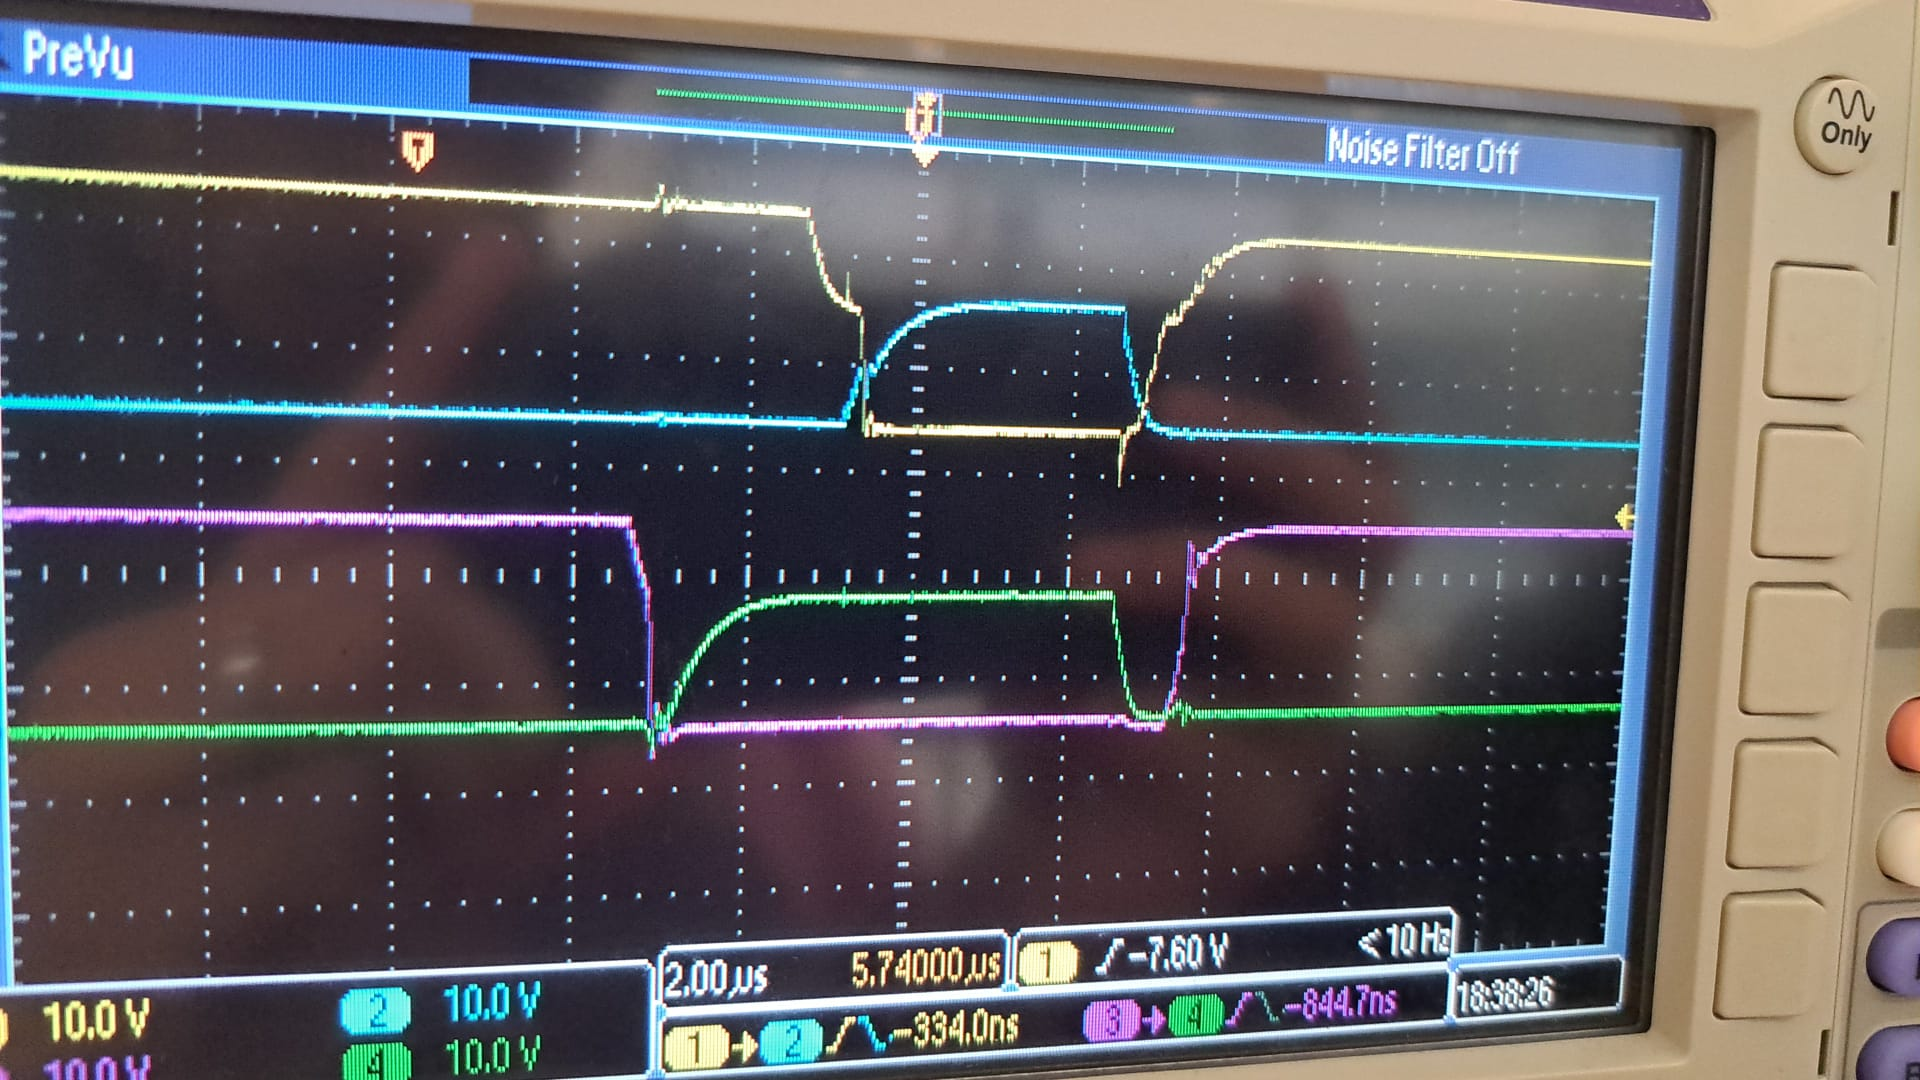
\includegraphics[width=\linewidth]{img//GateDriver/WhatsApp Image 2024-03-18 at 18.38.31_9fd81adb.jpg}
        \caption{Boven 5 ohm, onder 1 ohm.}
         \label{fig:smallshort}
    \end{subfigure}
    \hfill
    \begin{subfigure}{0.32\textwidth}
    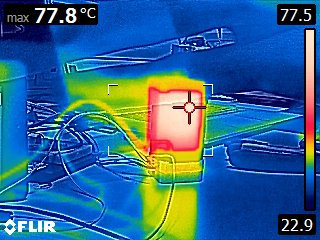
\includegraphics[width=\linewidth]{img/WhatsApp Image 2024-03-28 at 18.31.53_bad388f9.jpg}
    \caption{Enter Caption}
    \label{fig:BLDCHEAT}
    \end{subfigure}
    \hfill
  \label{fig:Buck}
  \caption{Testing}
\end{figure}


\subsection{MOSFET}\label{MOSFET}
The MOSFETs selected for the circuit are the IPP015N04NF2S\cite{infineon-ipp015n04nf2s-datasheet}. These MOSFETs work flawless within our circuit, requiring minimal testing. With a voltage rating of 40V and a current rating of 193A, they are well-suited to operate effectively within our 24V system.

\subsection{Buck Converter}\label{Buck converter}
The buck converters were designed with WeBench, following a recommendation from Diego. Two buck converters were created with the TPS62932\cite{ti-tps62932-datasheet} IC: one to step down 24V to 12V for the gate driver and another to step down 24V to 5V for the STM32F411\cite{stm32-base-board}, user interface, and Hall sensors. Extensive simulations and testing were conducted, confirming the effectiveness of the design. Upon subjecting the buck converters to a load (refer to \autoref{fig:BuckLoad}) of \(\frac{3\times50\Omega}{150\Omega}=16\frac{2}{3}\Omega\), both simulation and test results exhibited close correlation. Additionally, temperature readings (refer to \autoref{fig:BuckTemp}) revealed that the buck converter under this high load condition could reach elevated temperatures over prolonged periods of operation. An heatsink might be smart in the future.
\begin{figure}[H]
    \centering
    \hfill
    \begin{subfigure}{0.23\textwidth}
        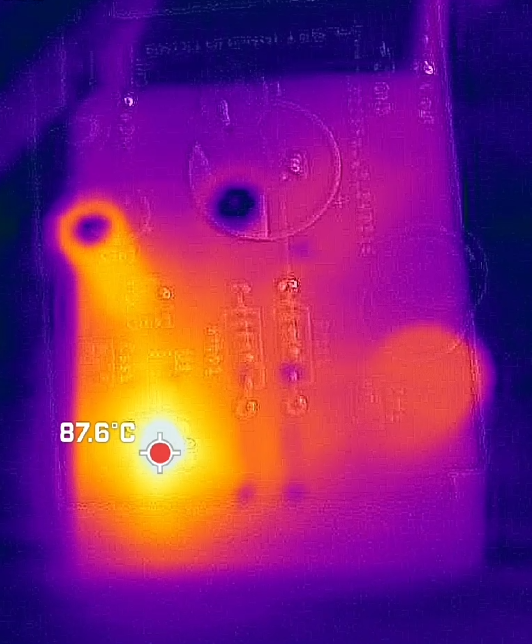
\includegraphics[width=\linewidth]{afbeelding2.png}
        \caption{Temp reading: Buck converter IC after 10min with load}
        \label{fig:BuckTemp}
    \end{subfigure}
    \hfill
    \begin{subfigure}{0.3\textwidth}
        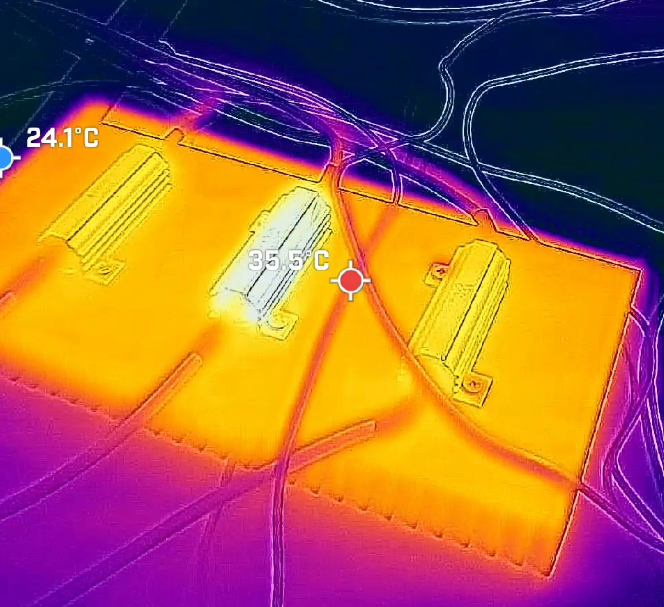
\includegraphics[width=\linewidth]{afbeelding.png}
    \caption{Temp reading: Buck converter load \(16\frac{2}{3}\Omega\).}
    \label{fig:BuckLoad}
    \end{subfigure}
    \hfill
  \label{fig:Buck}
  \caption{Buck converter testing}
\end{figure}



\subsection{BLDC}\label{BLDC}
Following thorough testing, it was observed that the hall sensors were not transmitting data as desired. Subsequently, a different motor was employed, yielding improved results. The feedback loop from our code to the gate drivers behaved as anticipated. Initially, it was not suspected that the motor itself was faulty. The defective BLDC motor\cite{reichelt-motor-datasheet} was entrusted to Stephen for further analysis, and a replacement motor was obtained, which functioned flawlessly.
\subsubsection{Temperature}
We have done some extensive testing into current drawnings. We have set the BLDC motor\cite{reichelt-motor-datasheet} under a load to see what would happend. We concluded that as the datasheet has given we motor indeed doens't have a lot of torque. Also we have done a lot of temperature measurements which resulted us in us changing code/hardware. We realized we were getting a short as told in \autoref{Gate driver}

\subsection{Interface}\label{Interface}
A decision was made to utilize a Raspberry Pi\cite{raspberrypi-3b} as the front-end interface\cite{sossolutions-7inch-touchscreen}. Establishing a rapid communication method was a priority, leading to the adoption of the I\textsuperscript{2}C protocol. Encounter of issues arose when the STM32F411\cite{stm32-base-board} struggled to receive the data, prompting the connection of pins to an oscilloscope to verify signal transmission. Upon confirmation that the issue was software-related, appropriate adjustments were made to resolve it.

\subsubsection{Current sensing}\label{Current Sensing}
In response to the project lead's requirement, we selected the INA181A3QDBVRQ1\cite{ti-ina181-q1} for current sensing, utilizing it alongside a shunt resistor to measure BLDC motor\cite{reichelt-motor-datasheet} current. This automotive-grade amplifier converts current to voltage for the STM32\cite{stm32-base-board} ADC to read. However, we recognized the potential for improvement and decided to explore the INA236BIDDFR\cite{ti-ina236-datasheet}, offering a 16-bit ADC interface via I\textsuperscript{2}C, providing significantly higher resolution than the STM32F411's\cite{stm32-base-board} 12-bit ADC. This upgrade promises enhanced accuracy with \(2^{16}-2^{12}=61440\) additional data points, although testing of this configuration is pending.
% \section{Hall sensor}\label{section:hallsensor}
\subsection{What is a hall sensor?}
A Hall sensor is a transducer that varies its output voltage in response to changes in the magnetic field. It is often used to detect the presence or absence of a magnetic field and to measure the strength and polarity of the field. The Hall sensor operates on the principle of the Hall effect, where a voltage difference is created across a conductor when it is subjected to a magnetic field perpendicular to the current flow.\cite{9568879}

\subsection{What does a hall sensor do in our application?}
In our application, the Hall sensors play a crucial role in providing feedback on the rotor position of the Brushless Direct Current (BLDC) motor. The three Hall sensors are strategically placed around the motor to detect the magnetic field generated by the rotating magnets in the rotor. By monitoring the Hall sensor outputs, we can determine the rotor's position, allowing precise control of the motor and enabling closed-loop operation.\cite{7489411}

\subsection{Hardware}
For the hardware setup, initial attempts to read out values on the oscilloscope were unsuccessful. After consulting with Diego Zuidervliet\cite{zuidervliet2024}, it was suggested to add either a pull-up or pull-down resistor to stabilize the Hall sensor outputs.

A pull-up resistor connects the sensor output to a high voltage level, and a pull-down resistor connects it to a low voltage level. The purpose is to ensure a defined voltage level when the sensor is not actively providing a signal. In our case, we added a 10K ohm pull-up resistor to each Hall sensor output.

The wiring diagram, shown in \autoref{fig:hall_sensor_wiring_diagram}, depicts the connection of the pull-up resistors to the Hall sensor outputs. With this modification, we successfully plotted the Hall sensor information on the oscilloscope, providing stable and readable output.

\begin{figure}[H]
    \centering
    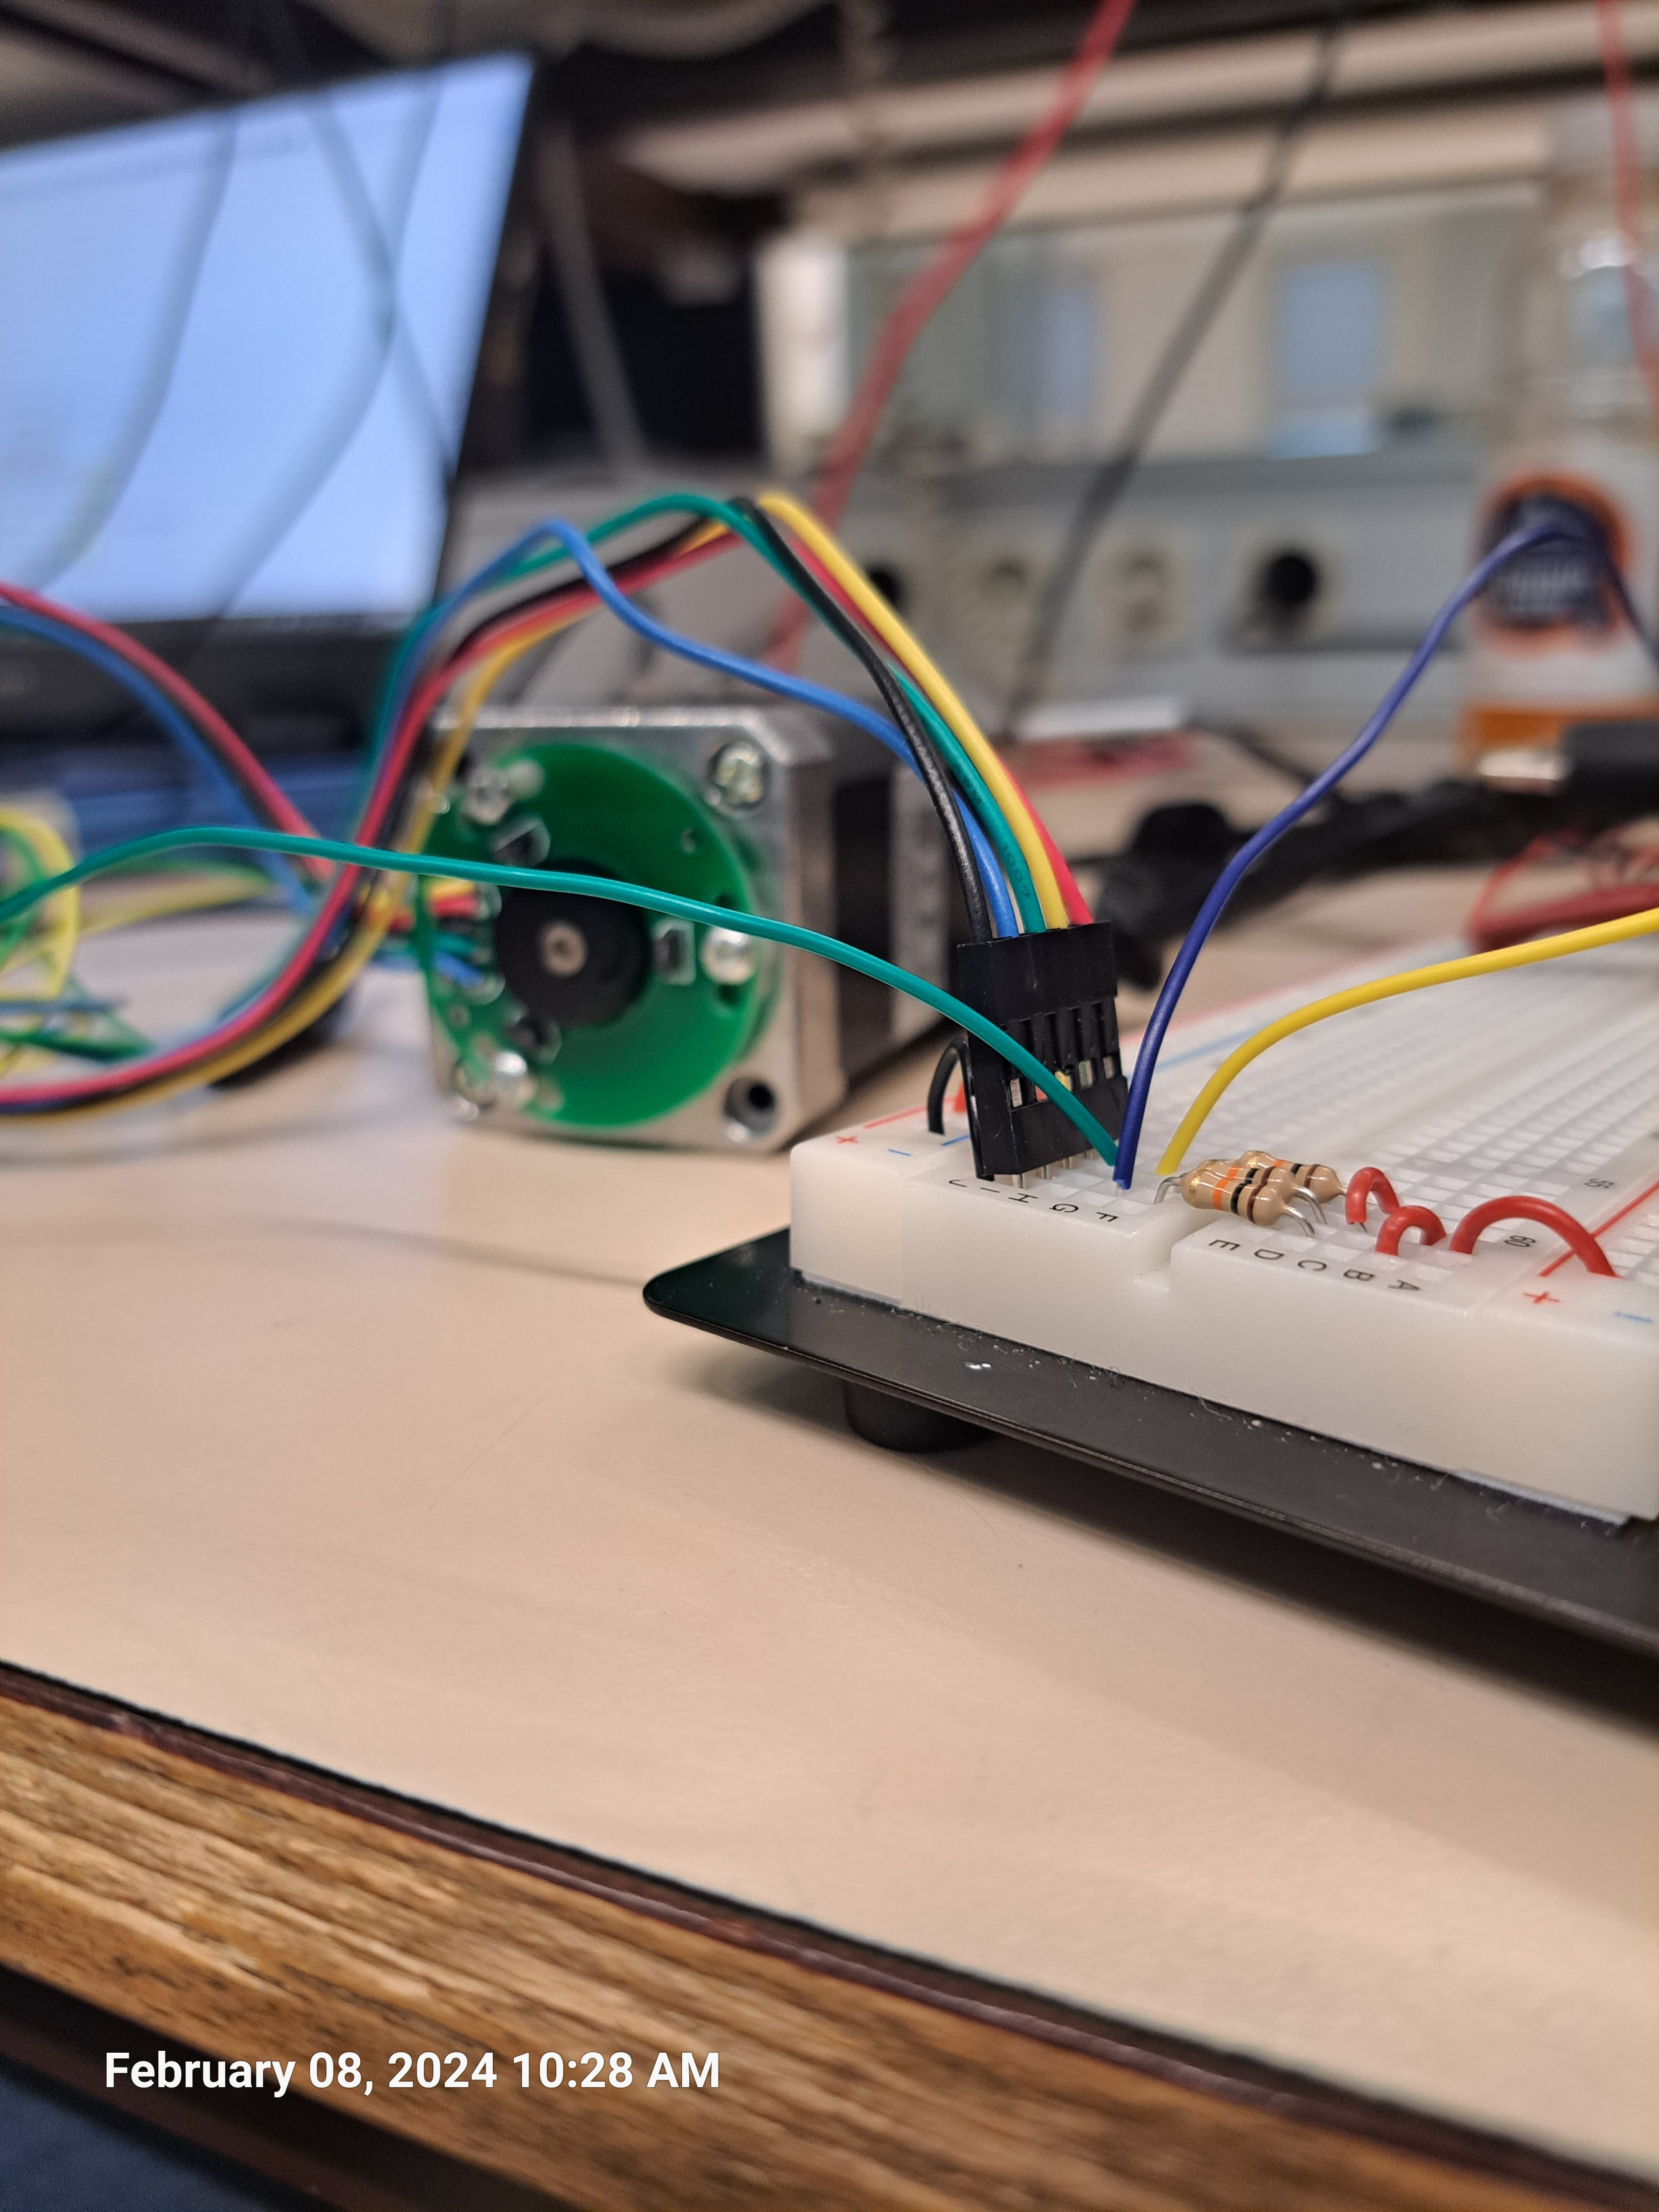
\includegraphics[width=0.3\textwidth]{img/Testing_Hallsensor_8-2-2024/Pictures/pull-up-resistor-breadboard-and-hall-sensor2.jpg}
    \caption{Wiring Diagram with Pull-up Resistors}
    \label{fig:hall_sensor_wiring_diagram}
\end{figure}

The circuit diagram, shown in \autoref{fig:hall_sensor_circuit_diagram}, illustrates the connection of the Hall sensors with the pull-up resistors.

\begin{figure}[H]
    \centering
    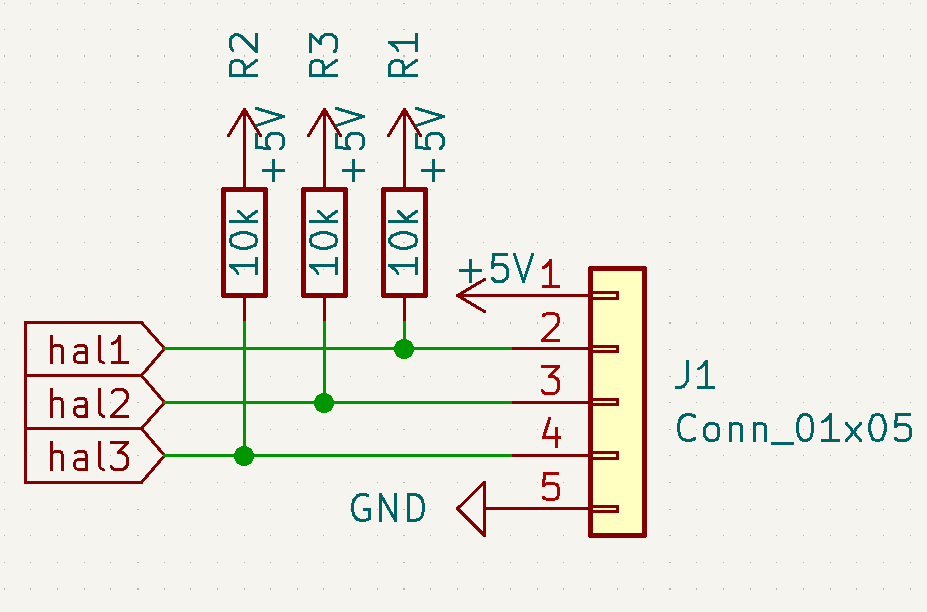
\includegraphics[width=0.45\textwidth]{img/Testing_Hallsensor_8-2-2024/Circuit/hall_sensor_circuit.png}
    \caption{Circuit: Hall sensor pinout with Pull-up Resistors}
    \label{fig:hall_sensor_circuit_diagram}
\end{figure}

Since we now understand the Hall sensor's function, its role in our application, and how to obtain stable readings, we can proceed with the software development.

\subsection{Software}
Using the Hall sensor input data we can determine the required ON/OFF states of the MOSFETS in the half bridges. This can be done using the build in HAL sensor functions as in \autoref{lst:HALFunction} or using registers as in \autoref{lst:Registers}. These listings will be further explained in \autoref{subsubsection:HALFunctions} and \autoref{subsubsection:Registers} 

The outputs from these listings are determined by \autoref{table:HallInput_Output} this is a diagram with the six Hall sensor states in time order and the output needed to the IN pin of the gate driver. The Out sections in this table contain the same data but have a different layout for better overview of the data.
\subsubsection{HAL functions}
\label{subsubsection:HALFunctions}
Using the HAL functions build into the STM32 we can with existing functions write ON/OFF states to the gate driver. This is achieved by first setting the HALPrevU - W variables on startup and after this to set the correct output equal to the previous input from the correct Hall sensor as shown in \autoref{lst:HALFunction}. For example for the output to Phase U the input from Hall W will be used. This is visualised in \autoref{table:HallInput_Output}

The benefit of using this method is simplicity and ease of use. This however comes at the cost of time, it takes significantly longer to write all necessary data than when using registers.

\subsubsection{Registers}
\label{subsubsection:Registers}
Another method to manipulate the output data to the gate driver is by directly changing the output data register of the correct GPIO port in this case port C. To load the correct data into this register the data from the input register of GPIO port B will be read an shifted to the correct pin numbers.

\autoref{lst:Registers} contains the code necessary to achieve this. First the Output Data Register (ODR) is set to the previous input data of the Hall sensors. After this the HALPrev variable will be set to the current input data shifted 8 bits to the left as the input data is on pins 5 to 7 and the output pins are 13 to 15.

The drawback of this method is the lack of simplicity. The troubleshooting and comprehending of the code will become much more difficult compared to using HAL functions.

\begin{table}[H]
\centering
\resizebox{\textwidth}{!}{%
\begin{tabular}{|ccc|c|ccc|c|ccc|}
\hline
\multicolumn{1}{|c|}{\cellcolor[HTML]{C0C0C0}\textbf{HallU}} &
  \multicolumn{1}{c|}{\cellcolor[HTML]{C0C0C0}\textbf{HallV}} &
  \cellcolor[HTML]{C0C0C0}\textbf{HallW} &
   &
  \multicolumn{1}{c|}{\cellcolor[HTML]{C0C0C0}\textbf{OutU}} &
  \multicolumn{1}{c|}{\cellcolor[HTML]{C0C0C0}\textbf{OutV}} &
  \cellcolor[HTML]{C0C0C0}\textbf{OutW} &
   &
  \multicolumn{1}{c|}{\cellcolor[HTML]{C0C0C0}\textbf{OutW}} &
  \multicolumn{1}{l|}{\cellcolor[HTML]{C0C0C0}\textbf{OutU}} &
  \multicolumn{1}{l|}{\cellcolor[HTML]{C0C0C0}\textbf{OutV}} \\ \cline{1-3} \cline{5-7} \cline{9-11} 
\multicolumn{1}{|c|}{1} &
  \multicolumn{1}{c|}{0} &
  1 &
   &
  \multicolumn{1}{c|}{0} &
  \multicolumn{1}{c|}{1} &
  0 &
   &
  \multicolumn{1}{c|}{0} &
  \multicolumn{1}{c|}{0} &
  1 \\ \cline{1-3} \cline{5-7} \cline{9-11} 
\multicolumn{1}{|c|}{1} &
  \multicolumn{1}{c|}{0} &
  0 &
   &
  \multicolumn{1}{c|}{0} &
  \multicolumn{1}{c|}{1} &
  1 &
   &
  \multicolumn{1}{c|}{1} &
  \multicolumn{1}{c|}{0} &
  1 \\ \cline{1-3} \cline{5-7} \cline{9-11} 
\multicolumn{1}{|c|}{1} &
  \multicolumn{1}{c|}{1} &
  0 &
   &
  \multicolumn{1}{c|}{0} &
  \multicolumn{1}{c|}{0} &
  1 &
   &
  \multicolumn{1}{c|}{1} &
  \multicolumn{1}{c|}{0} &
  0 \\ \cline{1-3} \cline{5-7} \cline{9-11} 
\multicolumn{1}{|c|}{0} &
  \multicolumn{1}{c|}{1} &
  0 &
   &
  \multicolumn{1}{c|}{1} &
  \multicolumn{1}{c|}{0} &
  1 &
   &
  \multicolumn{1}{c|}{1} &
  \multicolumn{1}{c|}{1} &
  0 \\ \cline{1-3} \cline{5-7} \cline{9-11} 
\multicolumn{1}{|c|}{0} &
  \multicolumn{1}{c|}{1} &
  1 &
   &
  \multicolumn{1}{c|}{1} &
  \multicolumn{1}{c|}{0} &
  0 &
   &
  \multicolumn{1}{c|}{0} &
  \multicolumn{1}{c|}{1} &
  0 \\ \cline{1-3} \cline{5-7} \cline{9-11} 
\multicolumn{1}{|c|}{0} &
  \multicolumn{1}{c|}{0} &
  1 &
   &
  \multicolumn{1}{c|}{1} &
  \multicolumn{1}{c|}{1} &
  0 &
   &
  \multicolumn{1}{c|}{0} &
  \multicolumn{1}{c|}{1} &
  1 \\ \cline{1-3} \cline{5-7} \cline{9-11} 
\multicolumn{3}{|c|}{\cellcolor[HTML]{EFEFEF}\textit{Hall}} &
  \multirow{-8}{*}{} &
  \multicolumn{3}{c|}{\cellcolor[HTML]{EFEFEF}\textit{Out}} &
  \multirow{-8}{*}{} &
  \multicolumn{3}{c|}{\cellcolor[HTML]{EFEFEF}\textit{Out}} \\ \hline
\end{tabular}%
}
\caption{Hall Input Output Diagram}
\label{table:HallInput_Output}
\end{table}

\begin{lstlisting}[caption={Set MOSFET ON/OFF states using HAL functions},label={lst:HALFunction},language=C]
    // Set new MOSFETS states
	HAL_GPIO_WritePin(GPIOC, GPIO_PIN_13, HALPrevW); // Set output U to previous HAL state W
	HAL_GPIO_WritePin(GPIOC, GPIO_PIN_14, HALPrevU); // Set output V to previous HAL state U
	HAL_GPIO_WritePin(GPIOC, GPIO_PIN_15, HALPrevV); // Set output W to previous HAL state V
	
	HALPrevU = HAL_GPIO_ReadPin(GPIOB, GPIO_PIN_5);
	HALPrevV = HAL_GPIO_ReadPin(GPIOB, GPIO_PIN_6);
	HALPrevW = HAL_GPIO_ReadPin(GPIOB, GPIO_PIN_7);	
\end{lstlisting}

\begin{lstlisting}[caption={Set MOSFET ON/OFF states using registers},label={lst:Registers},language=C]
    // Set new MOSFET states
    GPIOC->ODR |= HALPrev;
	HALPrev = GPIOB->IDR << 8;
\end{lstlisting}


% \section{Buck converter}
\subsection{What is a buck converter?}
A \textit{buck converter}, also known as a \textit{step-down converter}, is a type of DC-DC converter that efficiently converts a higher input voltage to a lower output voltage. The buck converter operates on the principle of pulse width modulation (PWM), controlling the duty cycle of the switch to regulate the output voltage.

\subsubsection{Applications}
Buck converters find widespread use in various electronic systems where it is necessary to step down voltage levels. They are commonly employed in power supplies for electronic devices, battery chargers, and voltage regulation circuits. Additionally, buck converters are frequently utilized in applications requiring efficient power management, such as in electric vehicles, renewable energy systems, and portable electronic devices where efficiency is a key component.

\subsection{What is the difference between a buck converter and a voltage regulator?}
The main differences between a \textit{buck converter} and a \textit{voltage regulator} lie in their operating principles, efficiency, and applications.

\begin{enumerate}
  \item \textbf{Operating Principle:}
    \begin{itemize}
      \item \textbf{Buck Converter:} Operates by switching the input voltage on and off at a high frequency, regulating the output voltage by controlling the duty cycle of the switch.
      \item \textbf{Voltage Regulator:} Adjusts the output voltage by dissipating excess energy as heat. The regulation is achieved through the use of linear components.
    \end{itemize}
  \item \textbf{Efficiency:}
    \begin{itemize}
      \item \textbf{Buck Converter:} Generally more efficient than voltage regulators, especially in scenarios where there is a significant voltage difference between the input and output.
      \item \textbf{Voltage Regulator:} Can be less efficient, particularly when dropping voltage by a large margin, as the excess energy is dissipated as heat.
    \end{itemize}
  \item \textbf{Cooling Requirement:}
    \begin{itemize}
      \item \textbf{Buck Converter:} Generates less heat due to its switching nature, often requiring less or no additional cooling elements.
      \item \textbf{Voltage Regulator:} Produces heat that needs to be dissipated, often requiring additional cooling elements such as heat sinks.
    \end{itemize}
  \item \textbf{Suitability for High Voltage Differences:}
    \begin{itemize}
      \item \textbf{Buck Converter:} Well-suited for applications with higher voltage differences, providing efficient voltage reduction.
      \item \textbf{Voltage Regulator:} Less suitable for high voltage differences due to increased heat dissipation and lower efficiency.
    \end{itemize}
\end{enumerate}


\subsection{What does a buck converter do in our application?}
In our application, which involves designing an electric bike motor, a \textit{buck converter} is employed to efficiently reduce voltage levels. This is crucial for optimizing the overall efficiency of the system. Diego Zuidervliet\cite{zuidervliet2024} recommended the use of Webench from Texas Instruments, a power simulator that simulated the creation of three different circuits utilizing the same switching IC: TI TPS62932DRLR.
\begin{figure}[H]
    \centering
    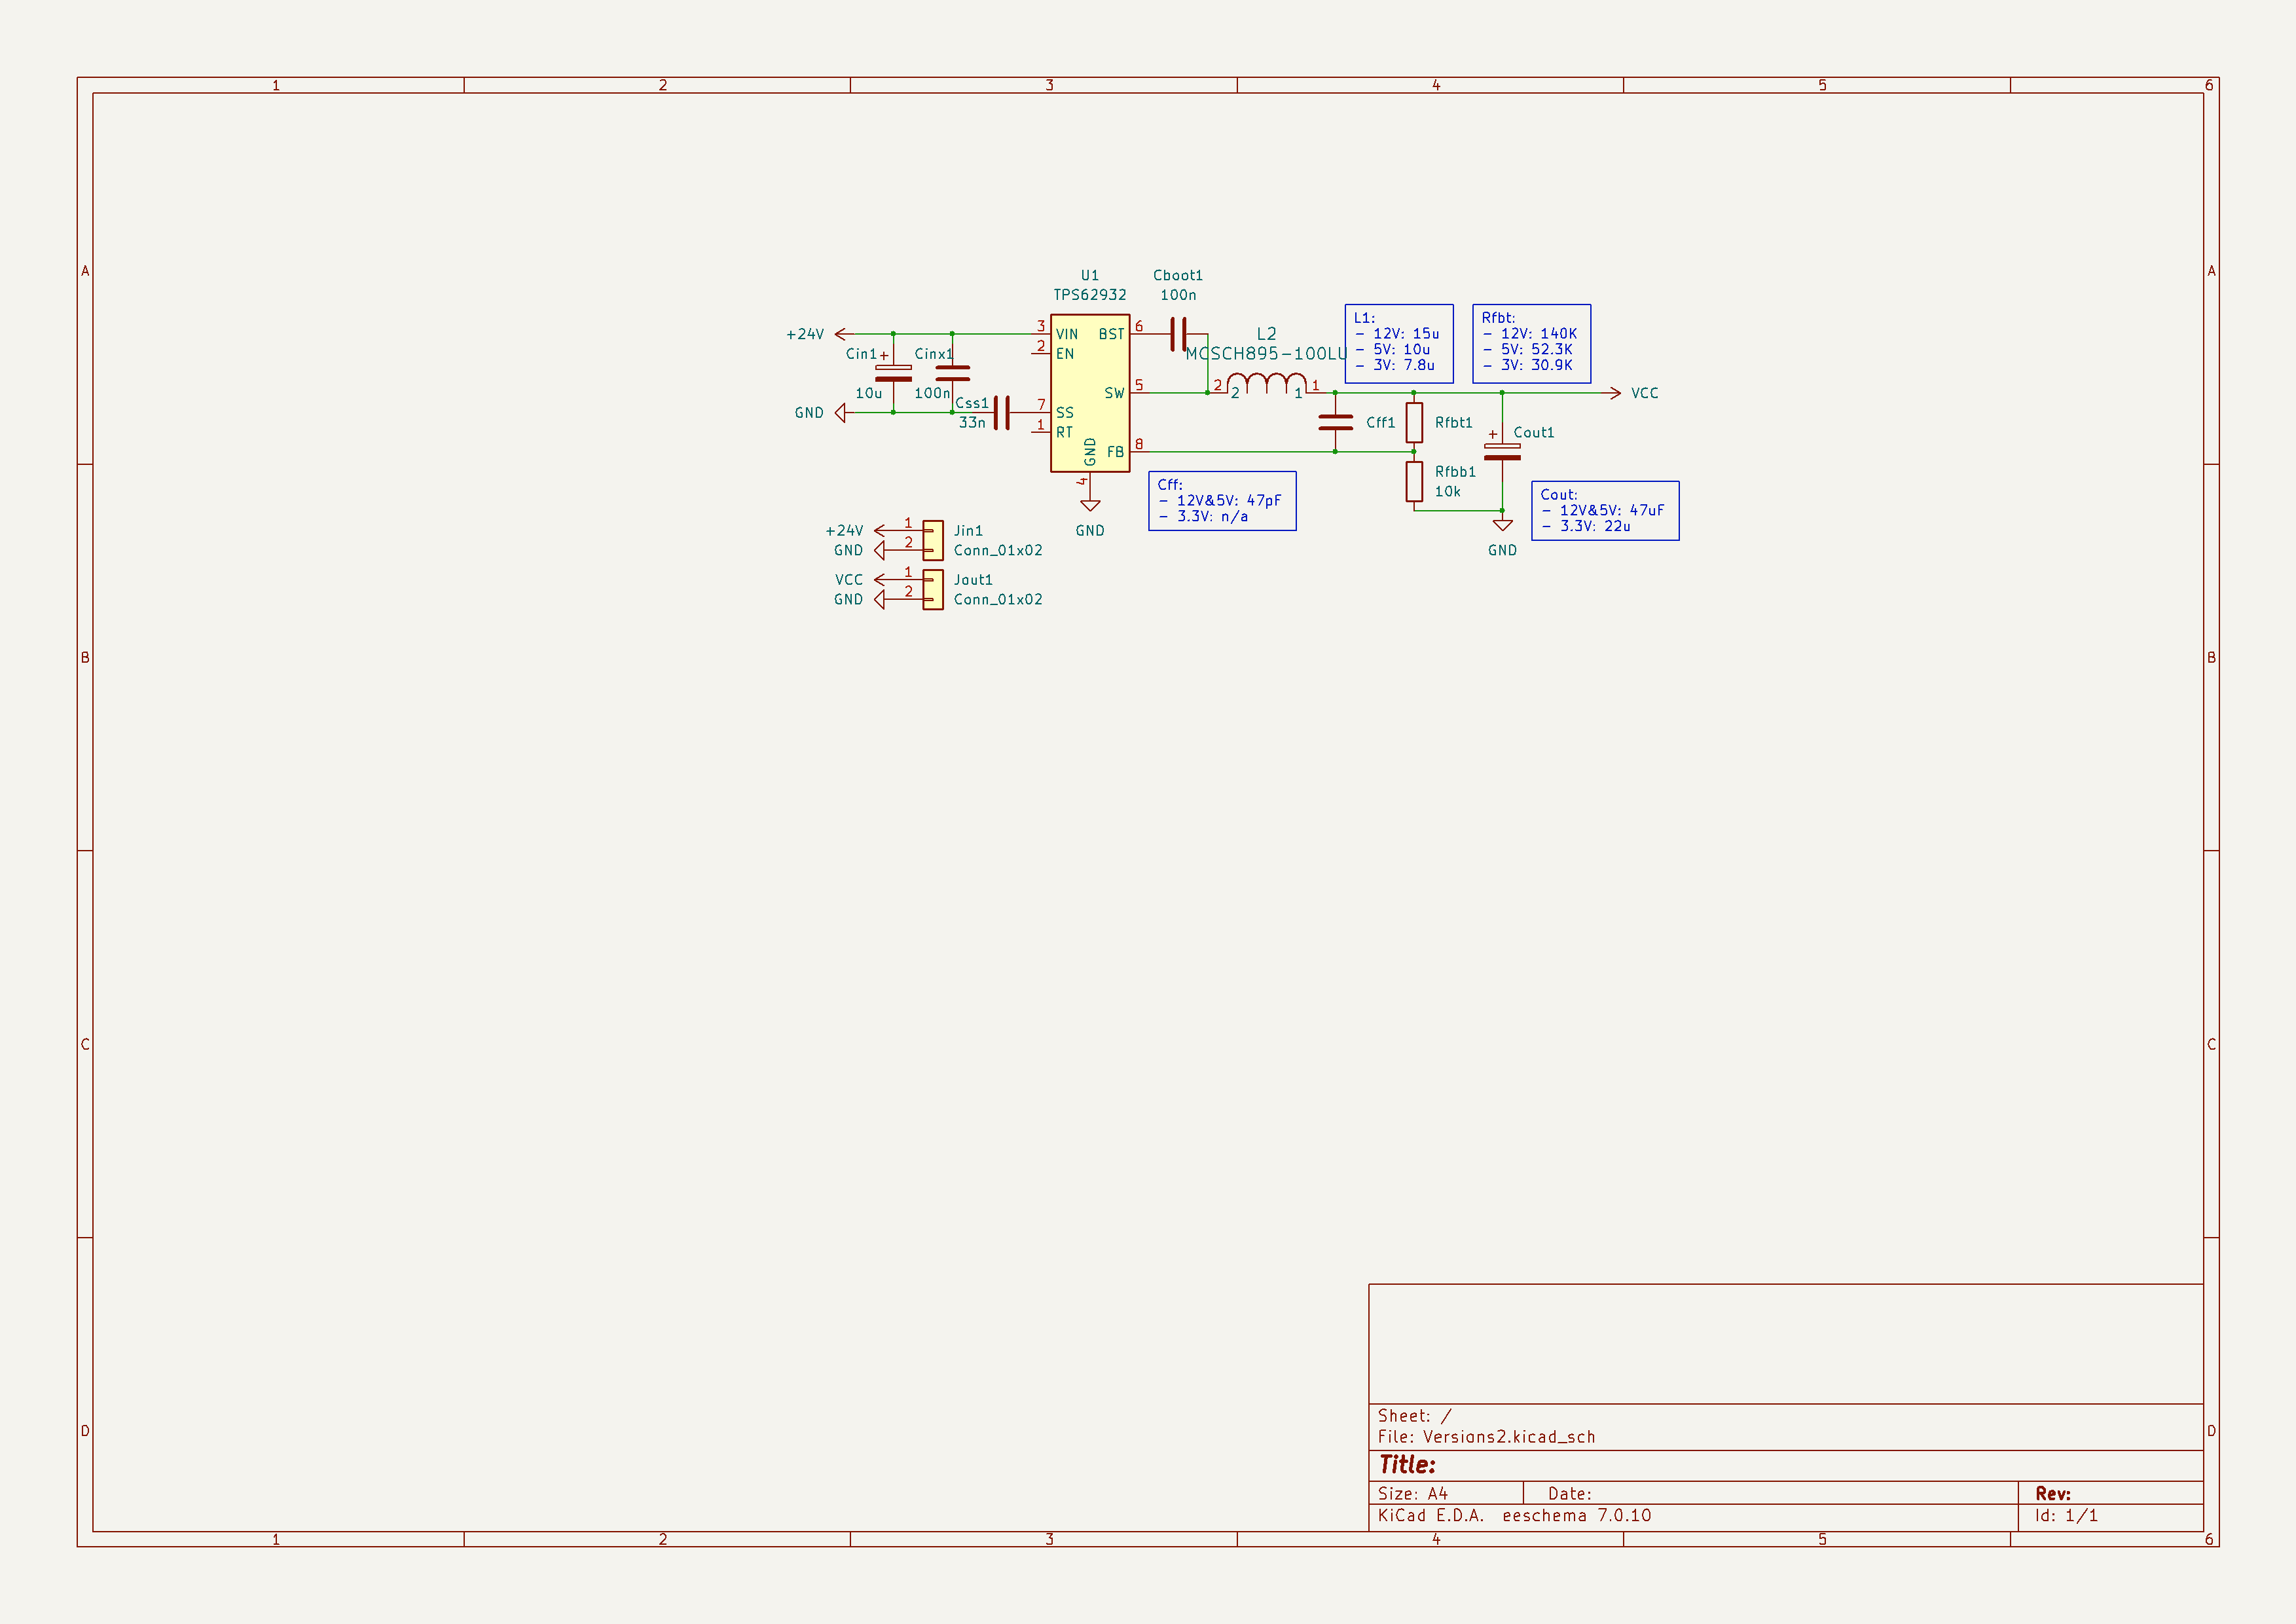
\includegraphics[trim=1150 1500 900 350,clip,width=0.8\linewidth]{img//buckconverters/circuit.png}
    \caption{Circuit: Versatile Buck converter}
    \label{fig:circuit_buck_converter}
\end{figure}
For testing purposes, a versatile circuit has been designed, allowing the generation of various voltages by making minor component changes, as depicted in \autoref{fig:circuit_buck_converter}. The decision to use a buck converter aligns with industry standards for dropping voltages efficiently. This approach ensures that the electric bike motor operates with high efficiency, a critical factor in achieving optimal performance and energy utilization in the context of an electrical bike motor.

\subsection{24V to 12V}
\subsubsection{Gate Driver Requirements}
Gate drivers play a crucial role in power electronics, facilitating the control of high-power semiconductor devices such as MOSFETs and IGBTs. In our system, the gate drivers are specified to operate within a voltage range of 10V to 20V. To meet this requirement, a 24V to 12V buck converter is employed to provide a stable and regulated 12V supply.

\autoref{section:gatedriver} provides additional details about the gate driver specifications.

\autoref{fig:buckconverter12v_VINVOUT} illustrates the voltage relationship between the input (24V) and output (12V) of the buck converter.
\begin{figure}[H]
    \centering
    \includegraphics[trim=0 235 0 70,clip,width=0.8\linewidth,page=8]{img//buckconverters//12v/WBDesign3.pdf}
    \caption{Buck converter 12V: Voltage in, Voltage out from: %\autoref{appendix:buckconverter}
    }
    \label{fig:buckconverter12v_VINVOUT}
\end{figure}

\subsubsection{Performance Analysis}
To ensure the reliability and stability of the 24V to 12V buck converter in our design, a series of simulations have been conducted. The following sections provide a detailed analysis of key performance aspects.

\subsubsection{Bode Plot Analysis}
The frequency response of the buck converter is analyzed through a Bode plot, as depicted in \autoref{fig:buckconverter12v_bodeplot}. This analysis provides insights into the converter's gain and phase margins, allowing us to assess its stability and transient response.
\begin{figure}[H]
    \centering
    \includegraphics[trim=0 165 0 70,clip,width=0.8\linewidth,page=8]{img//buckconverters//12v/WBDesign3_Bode Plot.pdf}
    \caption{Buck converter 12V: Bode plot Simulation from: %\autoref{appendix:buckconverter12v_bodeplot_full}
    }
    \label{fig:buckconverter12v_bodeplot}
\end{figure}

\subsubsection{Input Transient Simulation}
\autoref{fig:buckconverter12v_inputtransient} illustrates the response of the buck converter to input voltage transients. This simulation is crucial to evaluate the converter's ability to handle sudden changes in the input voltage and maintain stability during dynamic conditions.
\begin{figure}[H]
    \centering
    \includegraphics[trim=0 205 0 70,clip,width=0.8\linewidth,page=8]{img//buckconverters//12v/WBDesign3_Input Transient.pdf}
    \caption{Buck converter 12V: Input transient Simulation from: %\autoref{appendix:buckconverter12v_inputtransient_full}
    }
    \label{fig:buckconverter12v_inputtransient}
\end{figure}

\subsubsection{Load Transient Simulation}
The load transient simulation, shown in \autoref{fig:buckconverter12v_loadtransient}, assesses the converter's response to sudden changes in the output load. This is critical for ensuring that the converter can adapt and maintain a stable output voltage under varying load conditions.
\begin{figure}[H]
    \centering
    \includegraphics[trim=0 235 0 70,clip,width=0.8\linewidth,page=8]{img//buckconverters//12v/WBDesign3_Load Transient.pdf}
    \caption{Buck converter 12V: Load transient Simulation from: %\autoref{appendix:buckconverter12v_loadtransient_full}
    }
    \label{fig:buckconverter12v_loadtransient}
\end{figure}

\subsubsection{Startup Simulation}
The startup simulation, presented in \autoref{fig:buckconverter12v_startup}, examines the behavior of the buck converter during the initial power-up phase. It assesses the startup time and the stability of the output voltage during this crucial period.
\begin{figure}[H]
    \centering
    \includegraphics[trim=0 235 0 70,clip,width=0.8\linewidth,page=8]{img//buckconverters//12v/WBDesign3_Startup.pdf}
    \caption{Buck converter 12V: Startup Simulation from: %\autoref{appendix:buckconverter12v_startup_full}
    }
    \label{fig:buckconverter12v_startup}
\end{figure}

\subsubsection{Steady State Simulation}
\autoref{fig:buckconverter12v_SteadyState} illustrates the steady-state performance of the buck converter. This simulation confirms the converter's ability to provide a stable 12V output voltage under continuous operation.
\begin{figure}[H]
    \centering
    \includegraphics[trim=0 200 0 70,clip,width=0.8\linewidth,page=8]{img//buckconverters//12v/WBDesign3_Steady State.pdf}
    \caption{Buck converter 12V: Steady State Simulation from: %\autoref{appendix:buckconverter12v_SteadyState_full}
    }
    \label{fig:buckconverter12v_SteadyState}
\end{figure}

\subsubsection{Conclusion}
The 24V to 12V buck converter has been successfully designed to meet the power supply requirements of the gate drivers, operating in the specified range of 10V to 20V. Through comprehensive simulations, including Bode plot analysis, input and load transient simulations, startup, and steady-state simulations, the converter's performance has been thoroughly evaluated. The results demonstrate the converter's stability, reliability, and ability to maintain a constant output voltage under various operating conditions, ensuring optimal functionality of the gate drivers in our system.


\subsection{24V to 5V}
In the design and implementation of electronic systems, the need often arises to convert voltage levels to match the requirements of various components. This report addresses the specific task of converting a 24V input voltage to a 5V output voltage using a buck converter. The motivation behind this conversion is to provide a common voltage supply for components such as the hall sensor \autoref{section:hallsensor} (5V-20V), Raspberry Pi \autoref{section:interface} (5V), and touchscreen \autoref{section:interface}  (5V). The choice of 5V aligns with industry-standard operating voltages.

\subsubsection{Component Voltage Requirements}
The hall sensor, Raspberry Pi, and touchscreen in our system all operate at a common voltage of 5V. To ensure proper functionality and compatibility, a 24V to 5V buck converter is employed to provide a stable and regulated 5V supply.

\autoref{section:hallsensor}, \autoref{section:interface}, and \autoref{section:STM32F411CEU6} provide additional details about the specific components in the system.

\autoref{fig:buckconverter5v_VINVOUT} illustrates the relationship between the input (24V) and output (5V) voltages of the buck converter.
\begin{figure}[H]
    \centering
    \includegraphics[trim=0 235 0 70,clip,width=0.8\linewidth,page=3]{img//buckconverters//5v/WBDesign2.pdf}
    \caption{Buck converter 5V: Voltage in, Voltage out from: %\autoref{appendix:buckconverter5v_VINVOUT_full}
    }
    \label{fig:buckconverter5v_VINVOUT}
\end{figure}

\subsubsection{Performance Analysis}
To ensure the reliability and stability of the buck converter in our design, a series of simulations have been conducted. The following sections provide a detailed analysis of key performance aspects.

\subsubsection{Bode Plot Analysis}
The frequency response of the buck converter is examined through a Bode plot analysis, as depicted in \autoref{fig:buckconverter5v_bodeplot}. This analysis provides insights into the converter's gain and phase margins, allowing us to assess its stability and transient response.
\begin{figure}[H]
    \centering
    \includegraphics[trim=0 165 0 70,clip,width=0.8\linewidth,page=8]{img//buckconverters//5v/WBDesign2_Bode Plot.pdf}
    \caption{Buck converter 5V: Bode plot Simulation from: %\autoref{appendix:buckconverter5v_bodeplot_full}
    }
    \label{fig:buckconverter5v_bodeplot}
\end{figure}

\subsubsection{Input Transient Simulation}
\autoref{fig:buckconverter5v_inputtransient} illustrates the response of the buck converter to input voltage transients. This simulation is crucial to evaluate the converter's ability to handle sudden changes in the input voltage and maintain stability during dynamic conditions.
\begin{figure}[H]
    \centering
    \includegraphics[trim=0 205 0 70,clip,width=0.8\linewidth,page=8]{img//buckconverters//5v/WBDesign2_Input Transient.pdf}
    \caption{Buck converter 5V: Input transient Simulation from: %\autoref{appendix:buckconverter5v_inputtransient_full}
    }
    \label{fig:buckconverter5v_inputtransient}
\end{figure}

\subsubsection{Load Transient Simulation}
The load transient simulation, shown in \autoref{fig:buckconverter5v_loadtransient}, assesses the converter's response to sudden changes in the output load. This is critical for ensuring that the converter can adapt and maintain a stable output voltage under varying load conditions.
\begin{figure}[H]
    \centering
    \includegraphics[trim=0 235 0 70,clip,width=0.8\linewidth,page=8]{img//buckconverters//5v/WBDesign2_Load Transient.pdf}
    \caption{Buck converter 5V: Load transient Simulation from: %\autoref{appendix:buckconverter5v_loadtransient_full}
    }
    \label{fig:buckconverter5v_loadtransient}
\end{figure}

\subsubsection{Startup Simulation}
The startup simulation, presented in \autoref{fig:buckconverter5v_startup}, examines the behavior of the buck converter during the initial power-up phase. It assesses the startup time and the stability of the output voltage during this crucial period.
\begin{figure}[H]
    \centering
    \includegraphics[trim=0 235 0 70,clip,width=0.8\linewidth,page=8]{img//buckconverters//5v/WBDesign2_Startup.pdf}
    \caption{Buck converter 5V: Startup Simulation from: %\autoref{appendix:buckconverter5v_startup_full}
    }
    \label{fig:buckconverter5v_startup}
\end{figure}

\subsubsection{Steady State Simulation}
\autoref{fig:buckconverter5v_SteadyState} illustrates the steady-state performance of the buck converter. This simulation confirms the converter's ability to provide a stable 5V output voltage under continuous operation.
\begin{figure}[H]
    \centering
    \includegraphics[trim=0 200 0 70,clip,width=0.8\linewidth,page=8]{img//buckconverters//5v/WBDesign2_Steady State.pdf}
    \caption{Buck converter 5V: Steady State Simulation from: %\autoref{appendix:buckconverter5v_SteadyState_full}
    }
    \label{fig:buckconverter5v_SteadyState}
\end{figure}

\subsubsection{Conclusion}
The 24V to 5V buck converter has been successfully designed to meet the power supply requirements of the hall sensor, Raspberry Pi, and touchscreen, all operating at a common voltage of 5V. Through comprehensive simulations, including Bode plot analysis, input and load transient simulations, startup, and steady-state simulations, the converter's performance has been thoroughly evaluated. The results demonstrate the converter's stability, reliability, and ability to maintain a constant output voltage under various operating conditions, ensuring optimal functionality of the components in our system.


% \subsection{24V to 3.3V}
% In the design and operation of electronic systems, it is often necessary to convert voltage levels to match the requirements of specific components. In our case, the input voltage to an STM32 microcontroller is 3.3V, while the available power source provides 24V. This necessitates the use of a voltage regulator to step down the voltage from 24V to 3.3V. The chosen solution for this task is a buck converter.

% \subsubsection{STM32 Microcontroller Requirements}
% The STM32 microcontroller used in our application, specifically the STM32F411CEU6 model, requires a stable power supply of 3.3V. To meet this requirement, we employ a buck converter to step down the 24V input voltage to the desired 3.3V output voltage.

% \autoref{fig:buckconverter3v3_VINVOUT} illustrates the voltage relationship between the input (24V) and output (3.3V) of the buck converter.
% \begin{figure}[H]
%     \centering
%     \includegraphics[trim=0 235 0 70,clip,width=0.8\linewidth,page=7]{img//buckconverters//3v3/WBDesign4.pdf}
%     \caption{Buck converter 3.3V: Voltage in, Voltage out from: %\autoref{appendix:buckconverter3v3_VINVOUT_full}
%     }
%     \label{fig:buckconverter3v3_VINVOUT}
% \end{figure}

% \subsubsection{Buck Converter Performance Analysis}
% To ensure the reliability and stability of the buck converter in our design, various simulations have been conducted. The following sections provide an in-depth analysis of the key aspects of the buck converter's performance.


% \subsubsection{Bode Plot Analysis}
% The frequency response of the buck converter is crucial for understanding its stability and transient response. The Bode plot, shown in \autoref{fig:buckconverter3v3_bodeplot}, provides insights into the converter's gain and phase margins, allowing us to assess its stability under different operating conditions.
% \begin{figure}[H]
%     \centering
%     \includegraphics[trim=0 165 0 70,clip,width=0.8\linewidth,page=7]{img//buckconverters//3v3/WBDesign4_Bode Plot-5.pdf}
%     \caption{Buck converter 3.3V: Bode plot Simulation from: %\autoref{appendix:buckconverter3v3_bodeplot_full}
%     }
%     \label{fig:buckconverter3v3_bodeplot}
% \end{figure}

% \subsubsection{Input Transient Simulation}
% \autoref{fig:buckconverter3v3_inputtransient} depicts the response of the buck converter to input voltage transients. This simulation helps evaluate how well the converter handles sudden changes in the input voltage, ensuring stability during dynamic conditions.
% \begin{figure}[H]
%     \centering
%     \includegraphics[trim=0 205 0 70,clip,width=0.8\linewidth,page=7]{img//buckconverters//3v3/WBDesign4_Input Transient-3.pdf}
%     \caption{Buck converter 3.3V: Input transient Simulation from: %\autoref{appendix:buckconverter3v3_inputtransient_full}
%     }
%     \label{fig:buckconverter3v3_inputtransient}
% \end{figure}

% \subsubsection{Load Transient Simulation}
% In \autoref{fig:buckconverter3v3_loadtransient}, the load transient simulation illustrates the converter's response to sudden changes in the output load. This is a critical aspect of performance, ensuring the converter can adapt and maintain stable output voltage under varying load conditions.
% \begin{figure}[H]
%     \centering
%     \includegraphics[trim=0 235 0 70,clip,width=0.8\linewidth,page=5]{img//buckconverters//3v3/WBDesign4_Load Transient-2.pdf}
%     \caption{Buck converter 3.3V: Load transient Simulation from: %\autoref{appendix:buckconverter3v3_loadtransient_full}
%     }
%     \label{fig:buckconverter3v3_loadtransient}
% \end{figure}

% \subsubsection{Startup Simulation}
% The startup simulation, as shown in \autoref{fig:buckconverter3v3_startup}, examines the behavior of the buck converter during the initial power-up phase. It assesses the startup time and the stability of the output voltage during this critical period.
% \begin{figure}[H]
%     \centering
%     \includegraphics[trim=0 235 0 70,clip,width=0.8\linewidth,page=7]{img//buckconverters//3v3/WBDesign4_Startup-1.pdf}
%     \caption{Buck converter 3.3V: Startup Simulation from: %\autoref{appendix:buckconverter3v3_startup_full}
%     }
%     \label{fig:buckconverter3v3_startup}
% \end{figure}

% \subsubsection{Steady State Simulation}
% \autoref{fig:buckconverter3v3_SteadyState} illustrates the steady-state performance of the buck converter, confirming its ability to provide a stable 3.3V output voltage under continuous operation.
% \begin{figure}[H]
%     \centering
%     \includegraphics[trim=0 200 0 70,clip,width=0.8\linewidth,page=7]{img//buckconverters//3v3/WBDesign4_Steady State-4.pdf}
%     \caption{Buck converter 3.3V: Steady State Simulation from: %\autoref{appendix:buckconverter3v3_SteadyState_full}
%     }
%     \label{fig:buckconverter3v3_SteadyState}
% \end{figure}

% \subsubsection{Conclusion}
% The 24V to 3.3V buck converter has been successfully designed to meet the power supply requirements of the STM32 microcontroller. Through comprehensive simulations, including Bode plot analysis, input and load transient simulations, startup, and steady-state simulations, the converter's performance has been thoroughly evaluated. The results demonstrate the converter's stability, reliability, and ability to maintain a constant output voltage under various operating conditions, ensuring optimal functionality of the STM32 microcontroller in our application.
% \section{Gate driver} \label{section:gatedriver}

\subsection{What is a gate driver}
A \textit{gate driver} is an IC which applies logic to and amplifies its inputs. This allows for for example an MCU or other low powered circuits to drive MOSFETS at frequencies above 1kHz. In addition to this a gate driver allows the switching of a high side MOSFET in a half bridge which cannot be done without a gate driver and additional components. Depending on the driver a multitude of safety features can be used, such as the prevention of enabling both MOSFETS in a half bridge as this would cause a short-circuit.

\subsection{Hardware}
Our design will be using the IRS2004(S)PBF gate driver from Infineon \cite{IRS2004PBF_Datasheet}. This driver was chosen as it is available in a PDIP and SOIC package which allows for breadboard testing and PCB design without changing chips. The IRS2004 has two inputs IN and SD, the IN pin is used to select the active MOSFET, HIGH or LOW. The SD pin allows for PWM-control and disabling of the chip, this is achieved by disabling the outputs if LOW and enabling them if HIGH.

Due to the single input IN to select the active MOSFET it is impossible to activate both MOSFETS simultaneously due to an internal dead time which makes sure one MOSFET is disabled before the other is enabled.

\subsubsection{High side MOSFET}
To drive the HIGH side MOSFET of a half bridge a bootstrap capacitor and diode are required. These are required as the MOSFET needs a positive voltage across its gate and source pins. This is a problem as when the MOSFET is conducting the source voltage is equal to the drain voltage. This means a greater voltage than the drain voltage is required to drive the MOSFET. In our design the drain voltage equals the input voltage which is 24V while the gate drive operates on 12V. As such the gate to source voltage van never be positive when the MOSFET is conducting, as a result the MOSFET will turn off and stop conducting.

To overcome this problem a bootstrap capacitor is used to increase the gate to source voltage to the source voltage plus the gate driver supply voltage. This capacitor needs to be charged to function, it is therefore important to switch the MOSFET at 100kHz or more. To charge the bootstrap capacitor a diode is used. Both of these components are external and can thus be chosen as necessary. \autoref{fig:GateDriverConnection} displays a typical connection of a gate driver. The bootstrap diode and capacitor are connected to the Vb pin of the gate driver. In total there will be three of such circuits within our final PCB design.

\begin{figure}[H]
    \centering
    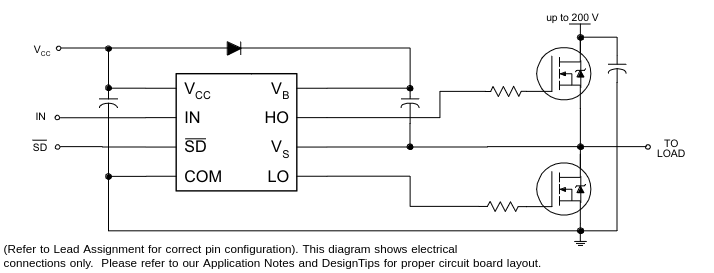
\includegraphics[width=0.5\textwidth]{img/GateDriver/Typical Connection Gate Driver.png}
    \caption{Typical Connection Gate Driver}
    \label{fig:GateDriverConnection}
\end{figure}

\subsection{Software}




% \begin{lstlisting}[caption={Start 3 PMW signals on timer 2 and mamage duty cycle},label={lst:STMSetup},language=C]
%     /* Initialize all configured peripherals */
%     MX_GPIO_Init();
%     MX_TIM2_Init();
%     MX_ADC1_Init();
%     MX_TIM1_Init();
%     MX_TIM3_Init();
%     /* USER CODE BEGIN 2 */

%     // Start PWM generation on three channels on timer 2
%     HAL_TIM_PWM_Start(&htim2, TIM_CHANNEL_1);
%     HAL_TIM_PWM_Start(&htim2, TIM_CHANNEL_2);
%     HAL_TIM_PWM_Start(&htim2, TIM_CHANNEL_3);

%     // If two timers are needed uncomment these
%     // HAL_TIM_PWM_Start(&htim3, TIM_CHANNEL_1);
%     // HAL_TIM_PWM_Start(&htim3, TIM_CHANNEL_2);
%     // HAL_TIM_PWM_Start(&htim3, TIM_CHANNEL_3);
%     // HAL_TIM_PWM_Start(&htim1, TIM_CHANNEL_1);
    
%     // Startup sequence
%     // Set active MOSFETS
%     HAL_GPIO_WritePin(GPIOC, GPIO_PIN_13, HAL_GPIO_ReadPin(GPIOB, GPIO_PIN_7)); // Set output U to HAL state W
%     HAL_GPIO_WritePin(GPIOC, GPIO_PIN_14, HAL_GPIO_ReadPin(GPIOB, GPIO_PIN_5)); // Set output V to HAL state U
%     HAL_GPIO_WritePin(GPIOC, GPIO_PIN_15, HAL_GPIO_ReadPin(GPIOB, GPIO_PIN_6)); // Set output W to HAL state V

%     // OR

%     GPIOC->ODR |= GPIOB->IDR << 8;;
    
%     /* USER CODE END 2 */
    
%     /* Infinite loop */
%     /* USER CODE BEGIN WHILE */
%     while (1)
%     {
    
%         HAL_ADC_Start(&hadc1);
%         HAL_ADC_PollForConversion(&hadc1, HAL_MAX_DELAY);
%         PWMPulse = HAL_ADC_GetValue(&hadc1) / 20;
    
%         /* USER CODE END WHILE */
    
%         /* USER CODE BEGIN 3 */
%     }
%     /* USER CODE END 3 */
% \end{lstlisting}

% See code \autoref{lst:STMSetup}.

% \begin{lstlisting}[caption={Read HAL ADC for PWM duty cycle control},label={lst:HalADC},language=C]
%     HAL_ADC_Start(&hadc1);
%     HAL_ADC_PollForConversion(&hadc1, HAL_MAX_DELAY);
%     PWMPulse = HAL_ADC_GetValue(&hadc1) / 20;
% \end{lstlisting}
% See code \autoref{lst:HalADC}.

% \begin{lstlisting}[caption={Interrupt routine using Hall sensor data},label={lst:stm32f4xx_it},language=C]
%     void EXTI9_5_IRQHandler(void)
%     {
%       /* USER CODE BEGIN EXTI9_5_IRQn 0 */
    
%     	//TIM2->CCR3 = HAL_GPIO_ReadPin(GPIOB, GPIO_PIN_5) * PWMPulse;
    
%     	// Save current state of Timers with new PWM duty cycle
%     	int PWMU = PWMPulse * CheckActive(TIM2->CCR1);
%     	int PWMV = PWMPulse * CheckActive(TIM2->CCR2);
%     	int PWMW = PWMPulse * CheckActive(TIM2->CCR3);
    
%     	// Set PWM duty cycle to zero for switching MOSFETS states
%     	TIM2->CCR1 = 0;
%     	TIM2->CCR2 = 0;
%     	TIM2->CCR3 = 0;
    
%     	// Set new MOSFETS states
%     	HAL_GPIO_WritePin(GPIOC, GPIO_PIN_13, HALPrevW); // Set output U to HAL state W
%     	HAL_GPIO_WritePin(GPIOC, GPIO_PIN_14, HALPrevU); // Set output V to HAL state U
%     	HAL_GPIO_WritePin(GPIOC, GPIO_PIN_15, HALPrevV); // Set output W to HAL state V
    
%     	HALPrevU = HAL_GPIO_ReadPin(GPIOB, GPIO_PIN_5);
%     	HALPrevV = HAL_GPIO_ReadPin(GPIOB, GPIO_PIN_6);
%     	HALPrevW = HAL_GPIO_ReadPin(GPIOB, GPIO_PIN_7);
    
%     	// OR
    
%     	GPIOC->ODR |= HALPrev;
%     	HALPrev = GPIOB->IDR << 8;
    
%     	// Set PWM duty cycle to previous saved state of preceding channel
%     	TIM2->CCR1 = PWMV;
%     	TIM2->CCR2 = PWMW;
%     	TIM2->CCR3 = PWMU;
    
%     	// Cycle through states
%     	/*int temp   = PWMPulse * CheckActive(TIM2->CCR1);
%     	TIM2->CCR1 = PWMPulse * CheckActive(TIM2->CCR2);
%     	TIM2->CCR2 = PWMPulse * CheckActive(TIM2->CCR3);
%     	TIM2->CCR3 = temp; */
    
%       /* USER CODE END EXTI9_5_IRQn 0 */
%       HAL_GPIO_EXTI_IRQHandler(GPIO_PIN_5);
%       HAL_GPIO_EXTI_IRQHandler(GPIO_PIN_6);
%       HAL_GPIO_EXTI_IRQHandler(GPIO_PIN_7);
%       /* USER CODE BEGIN EXTI9_5_IRQn 1 */
    
%       /* USER CODE END EXTI9_5_IRQn 1 */
%     }

%     /* USER CODE BEGIN 1 */

%     // Check if value is positive using simple IF-statement
%     int CheckActive(uint32_t x) {
%         if (x > 0) {
%             return 1;
%         } else {
%             return 0;
%         }
%     }
    
%     /* USER CODE END 1 */
% \end{lstlisting}
% See code \autoref{lst:stm32f4xx_it}.
% \section{MOSFET}
\begin{figure}[H]
    \centering
    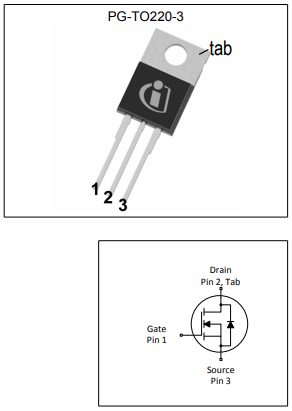
\includegraphics[width=0.5\textwidth]{img/MOSFET/MOSFET.png}
    \caption{IPP015N04NF2S}
    \label{fig:MOSFET:IPP015N04NF2S}
\end{figure}
For MOSFETs, three main factors are crucial: reliability, efficiency, and design. Reliability focuses on the device's limits, which must be prevented during operation. Efficiency refers to how much heat dissipation occurs.
Below, we outline the important aspects for the three main factors when choosing the MOSFET \cite{Proper-Specs-MOSFET}

\subsection{Reliability}
\begin{itemize}
    \item Suffice breakdown voltage protection
    \begin{itemize}
        \item In this case, with a 24 V BLDC motor, a MOSFET with a 40 V breakdown voltage would be sufficient.
    \end{itemize}
\end{itemize}

\subsection{Efficiency}
\begin{itemize}
    \item On-Resistance, $R_{ds(on)}$
    \item Gate charge, $Q_{g}$ 
    \item N-channel 
\end{itemize}

\subsection{Design}
\begin{itemize}
    \item Good thermal flow
    \item EMI
\end{itemize}


An N-channel MOSFET was chosen for implementation in the design. The selected type is the IPP015N04NF2S from Infineon, as shown in Figure \ref{fig:MOSFET:IPP015N04NF2S}. It has the following specifications \cite{Datasheet-MOSFET-IPP015N04NF2S} :
\begin{itemize}
    \item $V_{ds} = 40 V$
    \item $R_{ds(on),\text{max}} = 1.5 m\Omega$
    \item $I_{d} = 193 A$
    \item $Q_{oss} = 117 nC$
    \item $Q_{G}(0V..10V) = 106 nC$
\end{itemize}



% \section{Interface} \label{section:interface}
% \section{Current Sensing}
An important requirement set by the lead of the project was that we sense the current drawn by the BLDC motor. We choose for a `INA181A3QDBVRQ1`. this is an Automotive, Bidirectional, Low- and High-Side Voltage Output,
Current-Sense Amplifiers which needs a shunt resistor. Current sense resistors, or shunt resistors, are devices used to gauge the flow of current. They detect and convert current to a measured output voltage. Current sense resistors are generally low-value, high-power resistors. The IC will sent out an value which will be read buy the ADC of the STM32. 
\begin{figure}[H]
    \centering
    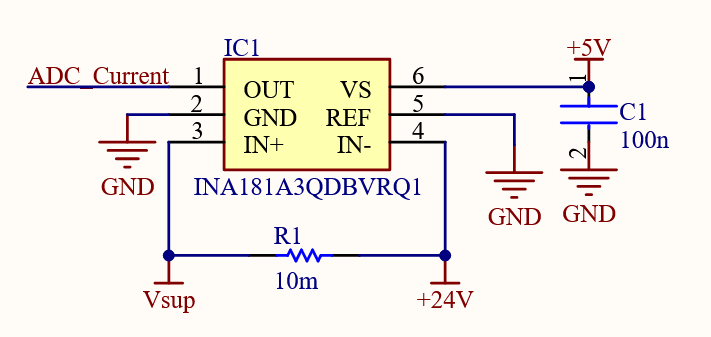
\includegraphics[width=0.5\linewidth]{img/Currentsense schem.png}
    \caption{Current sensing}
    \label{fig:Current sense Schem}
\end{figure}

Although this circuit may appear intriguing and effective, there is room for improvement. We opted for a different IC, the INA236BIDDFR, which is a 16-bit, Ultra-Precise Current, Voltage, and Power Monitor with an I\textsuperscript{2}C interface. This means that instead of utilizing the 12-bit ADC from the STM32F411, we now employ the 16-bit ADC from the INA236, allowing for \(2^{16}-2^{12}=61440\) additional data points, significantly enhancing accuracy. 
\begin{table}[H]
\begin{tabular}{|c|c|}
\hline
\rowcolor[HTML]{C0C0C0} 
\textbf{A0} & \textbf{INA236B DEVICE OPTION} \\ \hline
GND         & 1001000                        \\ \hline
VS          & 1001001                        \\ \hline
SDA         & 1001010                        \\ \hline
SCL         & 1001011                        \\ \hline
\end{tabular}
\end{table}
Furthermore, the measured values are transmitted via I\textsuperscript{2}C, providing flexibility in selecting the device address. We selected address 1001000 by connecting the \textbf{REF} to to \textbf{GND}, as it was available and not in use by our Raspberry Pi or Display.


% \section{Brushless DC}\label{section:BLDC}
% \section{PCB}





\subsection{Buck converter}
    \subsubsection{24V to 5V}
    
    
% \begin{lstlisting}[caption={Some C code},label={lst:label},language=C]
// Code...
\end{lstlisting}
See code~\ref{lst:label}.
% \section{Appendix}
\appendix
\includepdf[scale=0.8, pages=-,pagecommand={\label{appendix:buckconverter}}]{img/buckconverters/12v/WBDesign3.pdf}

\includepdf[scale=0.8, pages=-,pagecommand={\label{appendix:buckconverter12v_bodeplot_full}}]{img/buckconverters/12v/WBDesign3_Bode Plot.pdf}

\includepdf[scale=0.8, pages=-,pagecommand={\label{appendix:buckconverter12v_inputtransient_full}}]{img/buckconverters/12v/WBDesign3_Input Transient.pdf}

\includepdf[scale=0.8, pages=-,pagecommand={\label{appendix:buckconverter12v_loadtransient_full}}]{img/buckconverters/12v/WBDesign3_Load Transient.pdf}

\includepdf[scale=0.8, pages=-,pagecommand={\label{appendix:buckconverter12v_startup_full}}]{img/buckconverters/12v/WBDesign3_Startup.pdf}

\includepdf[scale=0.8, pages=-,pagecommand={\label{appendix:buckconverter12v_SteadyState_full}}]{img/buckconverters/12v/WBDesign3_Steady State.pdf}

\includepdf[scale=1, scale=0.8, pages=-,pagecommand={\label{appendix:buckconverter5v_VINVOUT_full}}]{img/buckconverters/5v/WBDesign2.pdf}

\includepdf[scale=0.8, pages=-,pagecommand={\label{appendix:buckconverter5v_bodeplot_full}}]{img/buckconverters/5v/WBDesign2_Bode Plot.pdf}

\includepdf[scale=0.8, pages=-,pagecommand={\label{appendix:buckconverter5v_inputtransient_full}}]{img/buckconverters/5v/WBDesign2_Input Transient.pdf}

\includepdf[scale=0.8, pages=-,pagecommand={\label{appendix:buckconverter5v_loadtransient_full}}]{img/buckconverters/5v/WBDesign2_Load Transient.pdf}

\includepdf[scale=0.8, pages=-,pagecommand={\label{appendix:buckconverter5v_startup_full}}]{img/buckconverters/5v/WBDesign2_Startup.pdf}

\includepdf[scale=0.8, pages=-,pagecommand={\label{appendix:buckconverter5v_SteadyState_full}}]{img/buckconverters/5v/WBDesign2_Steady State.pdf}

\includepdf[scale=1, scale=0.8, pages=-,pagecommand={\label{appendix:buckconverter3v3_VINVOUT_full}}]{img/buckconverters/3v3/WBDesign4.pdf}

\includepdf[scale=0.8, pages=-,pagecommand={\label{appendix:buckconverter3v3_bodeplot_full}}]{img/buckconverters/3v3/WBDesign4_Bode Plot-5.pdf}

\includepdf[scale=0.8, pages=-,pagecommand={\label{appendix:buckconverter3v3_inputtransient_full}}]{img/buckconverters/3v3/WBDesign4_Input Transient-3.pdf}

\includepdf[scale=0.8, pages=-,pagecommand={\label{appendix:buckconverter3v3_loadtransient_full}}]{img/buckconverters/3v3/WBDesign4_Load Transient-2.pdf}

\includepdf[scale=0.8, pages=-,pagecommand={\label{appendix:buckconverter3v3_startup_full}}]{img/buckconverters/3v3/WBDesign4_Startup-1.pdf}

\includepdf[scale=0.8, pages=-,pagecommand={\label{appendix:buckconverter3v3_SteadyState_full}}]{img/buckconverters/3v3/WBDesign4_Steady State-4.pdf}
 %% DEZE VERWIJDEREN MITS DIE FILE NIET MEER NODIG IS
\nocite{*}
\phantomsection
\addcontentsline{toc}{section}{References}
\printbibliography

% \appendix
% \input{appendix/python/motor_control.py} %vereist voor python opmaak
% \subsection{Specifications} \label{subsection:Specifications}
    \subsubsection{Microcontroller:}
    \begin{itemize}
        \item Part: STM32F411CEU6
        \item Manufacturer: ST-Microelectronics
        \item Core: Arm Cortex-M4
        \item Max. Clock Speed: 100MHz
        \item Package: UFQFPN 48 pins
    \end{itemize}

    \subsubsection{Internal Memories:}
    \begin{itemize}
        \item FLASH: 512KiB
        \item SRAM: 128KiB
    \end{itemize}

    \subsubsection{Oscillators:}
    \begin{itemize}
        \item HSI: 16MHz
        \item HSE: 25MHz (Critical for precise motor control)
        \item LSI: 32kHz
        \item LSE: 32.768kHz
    \end{itemize}

    \subsubsection{Power:}
    \begin{itemize}
        \item Voltage Input: +3.52V to +5.25V
        \item Power Sources: Any +3.3V pin, Any +5V pin, USB connector
        \item Backup battery: Supported
    \end{itemize}

    \subsubsection{Regulator:}
    \begin{itemize}
        \item Manufacturer: Diodes Incorporated
        \item Part: AP7343 (6T)
        \item Input: +3.52V to +5.25V
        \item Output: +3.3V @ 300mA
    \end{itemize}

    \subsubsection{PCB:}
    \begin{itemize}
        \item Color: Black
        \item Size (w x l): 20.78mm x 52.81mm
        \item Mounting: Breadboard
    \end{itemize}

    \subsubsection{Inputs \& Outputs:}
    \begin{itemize}
        \item Reset button (Active low)
        \item BOOT0 button (Active high)
        \item User button (Active low)
        \item Power LED (Connected to +3.3V rail)
        \item User LED (Connected to PC13)
    \end{itemize}

    \subsubsection{Connectors \& Headers:}
    \begin{itemize}
        \item Header 1 (20x1, male): 5V, GND, 3.3V, Motor Control Pins (PB0-PB10, PA0-PA7, PC13, NRST, PC15, PC14, VBAT)
        \item Header 2 (20x1, male): Motor Control Pins (PB12-PB15, PA8-PA15, PB3-PB9, 5V, GND, 3.3V)
        \item USB Connector (USB C): VBUS, D-, D+, GND (For potential external communication)
        \item SWD Header (4x1, male): 3.3V, SWDIO (PA13), SWCLK (PA14), GND (For debugging and programming)
    \end{itemize}

    \subsubsection{Devices:}
    \begin{itemize}
        \item Generic EEPROM (I2C): SOP 8 pins, Generic I2C EEPROM
        \item Connected to PA4 (CS), PB4 (DO), +3.3V rail (WP, HOLD), Ground plane (GND), PA7 (DI), PA5 (CLK), +3.3V rail (VCC)
    \end{itemize}

All data has been obtained from the listed sources.\cite{stm32datasheet,stm32base,stmicro}.

\end{document}
